% This is samplepaper.tex, a sample chapter demonstrating the
% LLNCS macro package for Springer Computer Science proceedings;
% Version 2.20 of 2017/10/04
%
\documentclass[envcountsect,runningheads]{llncs}

\usepackage{paralist}
\usepackage{graphicx}
\usepackage{epstopdf}
%\epstopdfDeclareGraphicsRule{.pdf}{png}{.png}{convert #1 \OutputFile}
\DeclareGraphicsExtensions{.pdf,.png}
\usepackage{subcaption}
\captionsetup{compatibility=false}
\let\proof\relax
\let\endproof\relax
\usepackage{amsthm}
\usepackage{amsmath}
\usepackage{amssymb}
\bibliographystyle{splncs04}
% Used for displaying a sample figure. If possible, figure files should
% be included in EPS format.
%
% If you use the hyperref package, please uncomment the following line
% to display URLs in blue roman font according to Springer's eBook style:
% \renewcommand\UrlFont{\color{blue}\rmfamily}
% Style de théorème sur mesure.
\newtheoremstyle{etoile}{\parskip}{\parskip}{\itshape}
                        {0pt}{\bfseries\sffamily}{.}{ }{}
\theoremstyle{etoile}
\def\proofname{\normalfont\bfseries\sffamily Proof}
\newcommand\bbox{\hfill\rule{2mm}{2mm}}
\let\qed=\bbox
% Les théoremes
\newtheorem{prop}{Proposition}[section]
\newtheorem{coro}[prop]{Corollaire}
\newtheorem{theo}[prop]{Theorem}
\newtheorem{defin}[prop]{Definition}
\newtheorem{lem}[prop]{Lemma}

\def\DD{\displaystyle}
\DeclareMathOperator*{\argmin}{argmin}
\DeclareMathOperator*{\argmax}{argmax}


\begin{document}
%
\title{Probabilistic Dynamic Time Lag: Predicting What \& When}
%
%\titlerunning{Abbreviated paper title}
% If the paper title is too long for the running head, you can set
% an abbreviated paper title here
%
\author{Mandar Chandorkar\inst{1,2} \and
Cyril Furtlehner\inst{2} \and
Bala Poduval \inst{4} \and
Enrico Camporeale\inst{1,3} \and 
Mich\`ele Sebag\inst{2}
}
%
\authorrunning{Chandorkar et al.}
% First names are abbreviated in the running head.
% If there are more than two authors, 'et al.' is used.
%
\institute{Centrum Wiskunde en Informatica, Amsterdam 1098XG, Netherlands \and
TAU, CNRS $-$ INRIA $-$ Univ. Paris-Saclay, France\and
CIRES, University of Colorado, Boulder, CO, USA \and 
University of New Hampshire, Durham, NH 03824, USA}
%
\maketitle              % typeset the header of the contribution
%
\begin{abstract}
      We formalize the joint regression task of predicting the magnitude of signals as well as the time delay with respect to their driving phenomena. 
      We call the problem \emph{probabilistic dynamic time lag} (PDT) to emphasize the uncertain and non-stationary time delay between the occurrence of 
      causes/drivers and the observation of effects in physical and man-made systems. We propose a solution to the PDT problem and a methodology to 
      benchmark and evaluate probabilistic time lag estimation algorithms.
\end{abstract}

\section{Introduction}
A significant body of work in machine learning concerns the modeling of spatio-temporal phenomena \cite{SurveyST}, 
ranging from markets \cite{Pedreschi} to weather forecasting \cite{Horvitz}.

This paper focuses on the problem of modeling the dependency between two series, 
where the latter one is {\em caused} by the former one \cite{Granger} with a non-stationary time delay. 

The motivating application domain is that of space weather.
The sun, a perennial source of charged energetic particles, is at the origin of a number of geomagnetic phenomena within the sun-earth system. 
Specifically, the sun ejects charged particles into the surrounding space in all directions and some of these particle clouds, a.k.a. solar winds, reach the earth vicinity. High speed solar wind is a major threat for the modern world, causing severe damages to e.g., satellites, telecommunication infrastructures, under sea pipelines, among others.\footnote{Economists have estimated that the adverse impact of space weather costs 200 to 400 millions per year, but can sporadically lead to much larger losses.} 
A key prediction task thus is to forecast the speed of the \emph{solar wind} in 
the vicinity of the Earth \cite{doi:10.1002/jgra.50429,doi:10.1029/2009SW000542}, sufficiently early to emit an alarm and be able to prevent the damages to the best possible extent.
Formally the goal is to model the dependency between the solar images (available at light speed), referred to as {\em cause series} 
and the solar wind speed series as recorded at the Lagrangian point $L_1$ (distant from the Earth by 1.5 million kilometers), referred to as {\em effect series}. 
The key difficulty is that the time lag between the solar images and the solar wind recorded at $L_1$ is {\em varying} depending on the initial direction of emitted particles and their energy. Would the lag be constant, the solar wind prediction problem would boil down to a mainstream regression problem. The challenge here (formalized in section \ref{sec:formulation})
is to predict, from the solar image $x[t]$ at time $t$ both {\em what} (the value of the solar wind speed) and {\em when} this solar wind speed will reach the earth: the task is to predict $y[t + \tau]$ where both the value $y$ and the time lag $\tau$ depend on $x[t]$. 


This challenge constitutes a new ML problem to our best knowledge. Indeed, the modeling of dependencies among financial time series has been intensively tackled (see \cite{ZHOU2006195} for instance). When considering varying time lag, the approaches rely on dynamic time warping (DTW) \cite{SakoeShiba1978}. For instance, DTW is used in \cite{SignalDiffusion}, taking a Bayesian approach to achieve the temporal alignment of both series; however the authors limit themselves to linear relationships between the cause and effect time series, and they further assume slow varying time lags. More generally, the use of DTW in time series analysis relies on simplifying assumptions on the cause and effect series (same dimensionality and structure) and build upon available cost matrices for the temporal alignment. 

This paper focuses on the identification of the varying time-lag phenomenon, considering synthetic problems involving increasingly more complex stochastic 
dependencies. The originality compared to the state of the art in DTW series alignment is threefold. Firstly, the cause and effect series are of different dimensionality. While the effect series is scalar, the cause series can be high-dimensional (e.g. images). Secondly, the relationship between the cause and the effect series can be non-linear (the {\em what} model). Thirdly, the time lag phenomenon (the {\em when} model) can be non smooth, as opposed to e.g. \cite{ZHOU2006195}.

The paper is organized as follows. Section \ref{sec:formulation} presents the formalization of the problem and the Bayesian analysis supporting the proposed learning criterion. Section \ref{sec:algo} describes the algorithm and the stability analysis. The experimental setting used to validate the approach is presented in section \ref{sec:expsetting}, and the proofs of concept of the approach are discussed in section \ref{sec:expe}. The paper concludes with some discussion for further work.


\section{Deterministic Formulation}\label{sec:formulation}

Time lag inference is essentially a regression problem with two tasks. 
Given two time series, the causes $x(t)$ and the observed effects $y(t)$, the regression model 
must learn a mapping $f(.)$ which maps each input pattern $x(t_1)$ to an output $y(t_2)$, and a 
mapping $g(.)$ which maps the time delay between the input and output patterns $t_2 = t_1 + g(x(t_1))$. 
This is formally specified in equations below.

\begin{align}
y(t + \tau(t)) & = f[x(t)]\label{eq:pb1}\\
\tau(t) & = g[x(t)]\label{eq:pb2} 
\end{align}
with
\[
f: \mathcal{X}  \rightarrow \mathbb{R},\qquad\text{and}\qquad
g: \mathcal{X}  \rightarrow \mathbb{R}^{+},
\]
$t \in \mathbb{R}^{+}$ represents the continuous temporal domain. The input signal 
$x(t)\in \mathcal{X}$ is possibly high dimensional and contains the hidden cause to 
the effect $y(t)\in\mathbb{R}$ which is considered as a scalar in this paper. 
$\tau(t)\in \mathbb{R}^+$ represents the time delay between inputs and outputs.

It is important to note some caveats about this time lag which make this inference problem 
different from classical time series regression problems.

Firstly, the time lag $\tau(t)$ can be \emph{non-stationary} i.e. dependent on the input $x(t)$. 
Secondly, in practical applications such as the motivating space weather example, $\tau(t)$ 
is not recorded explicitly in the training data. This makes model training and evaluation 
challenging.

One may make certain assumptions on the time warping function $\phi(t) = t + \tau(t)$, in the general 
formulation of the problem presented here: 

\begin{enumerate}
    \item $\phi(.)$ is assumed to be continuous and \emph{bijective}.
    \item Zhou \& Sornette \cite{ZHOU2006195} enforce further assumptions 
          such as $\phi(t_1) \leq \phi(t_2), \forall t_1 \leq t_2$, which 
          are incorporated via constraints. This approach respects the 
          properties associated with the warping function $\phi(.)$ but 
          increase the computational complexity of the resulting 
          optimization problem.
\end{enumerate}

The second assumption can be restrictive for applications in space physics, where fast moving 
solar wind can reach the Earth before slow moving solar wind which departed before it. 

In practical time-series applications, one works with sub-sampled or discretized versions of the time 
series $x(t)$ and $y(t)$. In this case the map $g(.)$ is replaced by its discrete analogue 
$g(.):\mathcal{X}  \rightarrow \mathbb{N}$. 

Henceforth we will work with the discretized time series $x^m$ and $y^m$.

\section{Probabilistic Formulation}\label{sec:probform}

Unlike the classical supervised learning problem, we cannot associate a time lagged output
$y^{m + i}$ and input $x^m$ with absolute certainty. It is therefore beneficial to relax 
the assumption of a deterministic time lag to a stochastic one. Our strategy consists of
learning a set of independent predictors $\{\hat y_i(x),i=1,\ldots n\}$ associated to a fixed time lag indexed by $i$, along with a set
of probabilistic weights $\{\hat p_i(x),i=1,\ldots n\}$ summing to one, indicating for a given input $x$ the probability for each time lag $i$
to be the correct one. These weights naturally arise from a latent variable model that we describe now.

\subsection{Latent model and associated likelihood}\label{sec:latent}

Suppose we discretize time in units of $\delta t$, such that for a given event $x^{(m)}$ at time  
$t = m\ \delta t$, the possible time lag $\tau^{(m)}$ is within a window $[\tau_{min},\tau_{max}]$. 
This interval is as well discretized into $n = (\tau_{max}-\tau_{min})/\delta t $ intervals so that 
the effect if any of this event has to be found in the vector of size $n$ of possible effects $(y^{(m+1)},\ldots,y^{(m+n)}\}$.
Assume now that for a given cause $x$ we are given a set of independent predictors $\{\hat y_i(x),i=1,\ldots n\}$ for these effects.
Our probabilistic formulation is based on the following conditional probability distribution:
\begin{equation}\label{eq:py}
  P\bigl[{\bf y}^{m} = {\bf y}\vert x^{(m)}=x\bigr] = \sum_{\{\tau_i\in\{0,1\}\}}  \hat p\bigl(\tau_1,\ldots,\tau_n\vert x)
\prod_{i=1}^n {\cal N}\bigl(\hat y_i(x),\sigma_i(\tau)\bigr)
\end{equation}
with 
\[
\sigma_i({\bf \tau})^{-2} = \Bigl(1+\sum_j\alpha_{ij} \tau_j\Bigr)\sigma^{-2},
\]
with $\sigma^2$ a default variance and $\alpha_{ij}\ge 0$ a matrix of non-negative real parameters. 
This is a local mixture model function of the input variable $x$. Its precise meaning is the following: for a given cause $x$ the effect
$y_i$ at horizon $i$ has a normal distribution centered on $\hat y_i(x)$ with  variance $\sigma_i^2({\bf \tau})$ (independent of $x$ as a simplifying assumption). $\{\tau_1,\ldots,\tau_n\}$ is a set of binary
latent variables encoding the stochastic causal time lag, telling whether $x$ causes $y_i$ ($\tau_i=1$) or not ($\tau_i=0$). Since we expect a one to one correspondence between causes
$x^{(m)}$ and effects $y^{m+i}$ we impose the constraint
\begin{equation}\label{eq:cs1}
\sum_{i=1}^n \tau_i = 1.
\end{equation}
The fact that $x$ can influence $y_i$ through the bias $\hat y_i(x)$ even when $\tau_i=0$ reflects an indirect
influence due to a finite auto-correlation time of $y_t$. But this should come with a higher variance, insured when $\alpha_{ij}$ is a decreasing function of $\vert i-j\vert$.
A large value of $\alpha_{ii}$ compared to $\alpha_{ij}$ for  $i\ne j$ 
should correspond to a small auto-correlation time. From the constraint~(\ref{eq:cs1}), $\hat p(\tau\vert x)$ is specified by  a vector
$\{\hat p_i(x),i=1,\dots n\}$ corresponding to
\[
\hat p_i(x) = \hat p(\tau_1=0,\ldots,\tau_i=1,\ldots,\tau_n=0\vert x),
\]
with 
\[
\sum_{i=1}^n \hat p_i(x) = 1.
\]
The log likelihood associated to this joint measure is: %(see appendix~\ref{app:LL}):
\begin{equation}\label{eq:LL}
{\cal L}\bigl[\hat {\bf y},\sigma,{\bf \alpha}] = -\frac{n}{2}\log(\sigma)-{\mathbb E}_{data}\Bigl[\frac{1}{2\sigma^2}\sum_{i=1}^n\bigl(y_i-\hat y_i(x)\bigr)^2
-\log\bigl(Z(\sigma,{\bf \alpha})\bigr)\Bigr],
\end{equation}
with
\[
Z(\sigma,{\bf \alpha}) = \sum_{i=1}^n\hat p_i(x)\exp\Bigl(-\frac{1}{2\sigma^2}\sum_j\alpha_{ji}\bigl(y_j-\hat y_j(x)\bigr)^2+\frac{1}{2}\sum_j\log(1+\alpha_{ji})\Bigr).
\]
Optimizing ${\cal L}$ yields the following expression of the optimal parameters:
\begin{equation}\label{eq:var}
\frac{\sigma^2}{1+\alpha_{ij}} = \frac{{\mathbb E}_{data}\bigl[\bigl(y_i-\hat y_i(x)\bigr)^2p_j(x,{\bf y})\bigr]}{{\mathbb E}_{data}\bigl[p_j(x,{\bf y})\bigr]},
\end{equation}
by means of the conditional probability $P(\tau_i=1\vert x,{\bf y})$ which reads
\begin{equation}\label{eq:hatpi}
p_i(x,{\bf y}) = \frac{1}{Z(\sigma,{\bf \alpha})}\hat p_i(x)\exp\Bigl(-\frac{1}{2\sigma^2}\sum_j\alpha_{ji}\bigl(y_j-\hat y_j(x)\bigr)^2+\frac{1}{2}\sum_j\log(1+\alpha_{ji})\Bigr).
\end{equation}
These are implicit equations, since ${\bf p}(x,{\bf y})$ depends on the parameters $\sigma^2$ and $\alpha_{ij}$.
In addition the optimal $\hat {\bf p}$ reads:%(see appendix~\ref{app:LL})
\begin{equation}\label{eq:tildep}
\hat p_i(x) = {\mathbb E}_{data,y}\Bigl[p_i(x,{\bf y})\Bigr].
\end{equation}

Practically the saddle point equations (\ref{eq:var},\ref{eq:hatpi},\ref{eq:tildep}) can be solved by alternatively updating $\hat {\bf p}$
and the parameters through equations~(\ref{eq:hatpi}) and~(\ref{eq:var}). The type of solution to be expected is analyzed in the next section,
in a simpler case where $\alpha_{ij} = \alpha\delta_{ij}$.


\subsection{Linear stability analysis}\label{sec:stability}
Let $\Delta y_i^2(x)= \bigl(y_i-\hat y_i(x)\bigr)^2$ and call
\[
\sigma_0^2 = \frac{1}{n}{\mathbb E}_{data}\Bigl(\sum_{i=1}^n \Delta y_i^2(x)\Bigr)
\]
the default mean square error of the predictor ${\hat {\bf y}}(x)$.
There is a degenerate solution to the saddle point equations (\ref{eq:var},\ref{eq:hatpi},\ref{eq:tildep}) corresponding to $\hat p_i(x) = 1/n$, $\alpha_{ij}=0$ for all
pairs $(i,j)$ with $\sigma^2=\sigma_0^2$. Intuitively the model could converge to this solution when the set of predictors are not specific enough.
It would be therefore interesting to identify the conditions under which this degenerate solution may appear. For this we can compute the Hessian and check its eigenvalues.
To simplify the analysis
we restrict the analysis to the set of parameters
\[
\alpha_{ij} = \alpha \delta_{ij},
\]
which leaves us with only two parameters $\alpha$ and $r = \sigma^2/\sigma_0^2$. Leaving aside the details of the computation, %for the Appendix~\ref{app:Hessian},
the situation can be summarized as follows. There are two key statistical quantities:
\begin{align}
C_1[{\bf p}] &= \frac{1}{\sigma_0^2}{\mathbb E}_{data}\Bigl(\sum_{i=1}^n p_i(x,{\bf y})\Delta y_i^2(x)\Bigr),\label{def:C1}\\[0.2cm]
C_2[{\bf p}] &= \frac{1}{\sigma_0^4}{\mathbb E}_{data}\Bigl[\sum_{i=1}^n p_i(x,{\bf y})\Bigl(\Delta y_i^2(x)-\sum_{j=1}^np_j(x,{\bf y})\Delta y_j^2(x)\Bigr)^2\Bigr].\label{def:C2}
\end{align}
$C_1$ represents the covariance between the latent variables $\{\tau_i\}$ and the normalized predictor errors. $C_1$ smaller than one 
indicates a positive correlation between the latent variables and small errors. At the degenerate point, i.e. ${\bf p}={\bf p}_{0}$ uniform, $C_1[{\bf p}_{0}]=1$ and $C_2[{\bf p}_{0}]$
represents the default variability among the predictor errors.
At a saddle point the parameters are given by:
\begin{align*}
\frac{\sigma^2}{\sigma_0^2} &= \frac{n-C_1[{\bf p}]}{n-1} \\[0.2cm]
\alpha &= \frac{n}{n-1}\frac{1-C_1[{\bf p}]}{C_1[{\bf p}]}.
\end{align*}
Such a saddle point is stable whenever
\[
C_2[{\bf p}] < 2C_1[{\bf p}]+{\cal O}\bigl(\frac{1}{n}\bigr).
\]
In particular the condition for the degenerate point to be unstable is
\[
C_2[{\bf p}_0] > 2\bigl(1-\frac{1}{n}\bigr).
\]
Note that for $\Delta y_i(x)$ iid centered with variance $\sigma_0^2$ and relative kurtosis $\kappa$ (conditionally to $x$)
we have $C_2 = (2+\kappa)(1-1/n)$. As a result, as soon as there are fluctuations among the $\Delta y_i^2(x)$ with non-negative relative kurtosis ($\kappa=0$ for a normal variable)
the  degenerate solution will be unstable.

\subsection{Loss function and related optimal predictor}
Once the set $\hat {\bf y}(x)$ of predictors is learned and assuming that the correct parameters for~(\ref{eq:py}) have been found
we would like to know for a given input $x$, what is the optimal predictor for $y_i(x)$. Any predictor has  to come in a composite form
$(\hat y(x),\hat I(x))$ where $\hat I(x)$ is the predicted index and $\hat y(x)$ the predicted value.
This is necessarily associated to a loss function 
which we specify with an $L_2$ norm:
\begin{equation}\label{eq:orloss}
{\cal L}(\hat y,\hat I) = {\mathbb E}_{data}\Bigl[\bigl(y_{\hat I(x)}-\hat y(x)\bigr)^2\Bigr]. 
\end{equation}
Then we have the following statement:
\begin{prop}\label{prop:opred}
Based on~(\ref{eq:py}), with $\alpha_{ij} = \alpha\delta_{ij},\ \alpha>0$, the optimal composite predictor $(y^\star,I^\star)$ is given by
\[
y^\star(x) = \hat y_{I^\star(x)}(x)\qquad\text{with}\qquad I^\star(x) = \argmax_{i} \bigl(\hat p_i(x)\bigr), 
\]
\end{prop}
\begin{proof}
See Appendix~\ref{app:opred}
\end{proof}

Since $\hat {\bf p}$ is self-consistently determined by~(\ref{eq:tildep}) along with equation~(\ref{eq:var}), what is needed from the practical point of view is to be able
to solve two  regression problems, namely $\hat {\bf y}(x)$ and $\hat {\bf p}(x)$ from a set of observations $\{(x^{m},{\bf y}^{m})\}$ with a given set of parameters ${\bf \alpha}$
and $\sigma^2$ in order then to be able to iterate the saddle point equations. The practical implementation of this framework will be described in the next section.


\section{Practical Solution}\label{sec:model}

\subsection{Neural network architecture}
From the practical point of view, the two aforementioned regression problems $\hat {\bf y}(x)$ and $\hat {\bf p}(x)$ can be solved efficiently with help of neural networks, with possibly deep
architectures depending on the dimension of the input signal $x$. Since the output $y$ and time lag $\tau$ have common causes we expect a single architecture with feature sharing
for $\hat {\bf y}(x)$ and $\hat {\bf p}(x)$ to be more efficient.
\begin{figure}[ht]
\centerline{\resizebox*{0.7\textwidth}{!}{\input{archi.pdf_t}}}
\caption{\label{fig:archi} Architecture of the neural network specified by the number of units $(n^v,n_1^h,n_2^h,2n)$ in each layer.}
\end{figure}
Beside the output layer which is constrained to be of size $2 \times n$ where $n$ is the chosen size of the time window,
the composition and size of the layers preceding the output layer are dependent on the application. 
One may choose \emph{convolutional layers} for input data which consists of images and fully connected 
layers for vector data.
In section \ref{sec:exp}, we use fully connected neural architectures sketched on Figure~\ref{fig:archi}, having a maximum depth of 
two hidden layers, for prediction of outputs and time lags. 
In order to train it we retro-propagate the following loss function:
\begin{equation}
\mathcal{L}(y^{(1:M)}, \hat{y}^{(1:M)}, \hat{p}^{(1:M)}) =
 \frac{1}{M}\sum_{i,m} \frac{1 + \alpha \hat{p}^{(m)}_i}{2\sigma^2}(y^{(m)}_{i} - \hat{y}^{(m)}_{i})^2   
+  \hat{p}^{(m)}_{i}\log \left (\frac{\hat{p}^{(m)}_i}{\tilde{p}^{(m)}_i} \right).\label{eq:loss}
\end{equation}
This function is computed over a mini-batch of size $M$ with $m=1\ldots M$ referring  to data sample indices within the
mini-batch in question. Its form is  adapted from the theoretical considerations discussed in the previous section in order to allow for feature sharing.
It can be considered as a convex relaxation of the loss function~(\ref{eq:orloss}). 
Parameters $\alpha$ and $\sigma^2$ have been already defined. From the variational point of view it can be checked that this form leads
each predictor $\hat y_i(x)$ to minimize a squared error independently of each other and of the other set of predictors $\hat {\bf p}$, while these are led to converge
to the form given in~(\ref{eq:tildep}).
$\tilde p(x)$ is an optional prior distribution, possibly based on expert knowledge, which corresponds to some initializing of $\hat p(x)$. 
In practice we use
\begin{equation}\label{eq:targetprob}
\widetilde{p}_{i}^{(m)} = \frac{\exp \left(- \beta (y_{i}^{(m)} - \hat{y}_{i}^{(m)})^{2} \right)}
{\sum_{i}{\exp \left(- \beta (y_{i}^{(m)} - \hat{y}_{i}^{(m)})^{2} \right)}} 
\end{equation}
with $\beta>0$ an additional parameter, which in the end correspond to the  shift $\alpha\to\alpha+\beta$.


\subsection{Hyper-parameters tuning}

Hyper-parameter selection is an important part of the model training process in the PDT problem. 
The hyper-parameter selection problem in deep learning has received much attention and a number 
of methodologies have been proposed for tacking it. 

Snoek et. al \cite{snoek2012practical} cast the problem in the formalism of Bayesian optimization, their method 
builds a Gaussian Process based surrogate model of the hyper-parameter fitness surface and computes 
updates based on expected improvement. 


Bergstra et. al \cite{hypBengio} demonstrate that sequential hyper-parameter search techniques yield state of the art 
results when applied on \emph{Deep Belief Nets} (DBN). 

Bergstra \& Bengio \cite{randomsearchBengio} showed that random search can be an effective way for tuning model 
hyper-parameters in several problem domains, and serve as a good baseline which can enable 
further improvement in model performance.

In the current work, we employ random search for hyper-parameter selection. 



\section{Experiments}\label{sec:exp}


Just as the MNIST, CIFAR Santa Fe Laser and other data sets serve as a way to evaluate machine learning 
algorithms, it is necessary to propose benchmark problems for \emph{Probabilistic Dynamic Time Lag}.

This is particularly challenging given the nature of the PDT problem, although time lag 
relationships do exist in real world data sets (\cite{doi:10.1002/jgra.50429}, \cite{ZHOU2006195}), 
it is difficult to find data sets with time lag relationships explicitly annotated.

This barrier can be surpassed in turn by careful construction of synthetic data sets which incorporate 
dynamic time lag relationships between causes and effects with various complexity.

Synthetic data sets allow us to evaluate the accuracy of both, the output and time lag predictions of 
PDT models. To this end, we propose four benchmark tests, which are motivated by their connection 
to the solar wind prediction problem, but which we hope can become canonical examples in the area 
of PDT modelling.

\subsection{Data Generation}

We start by generating the time series $x(t) \in \mathbb{R}^10$, 
which represent the driving forces in our system. This can be achieved with 
good flexibility using \emph{Stochastic Langevin Dynamics} as shown in 
equation \ref{eq:data}.

\begin{align}
 x(t + 1) &= (1 - \eta) x(t) + \mathcal{N}(0, s^2) \label{eq:data}\\
 y(t + \tau(t)) &= k ||x(t)||^2 + c \label{eq:outputs}
\end{align}

Equation \ref{eq:outputs} defines the output $y(.)$ as the square norm of the appropriately 
time lagged input, where $\tau(t)$ determines the time lag relationship.

In each benchmark we set $\eta = 0.02, s^2 = 0.7$, for the data generation process.


\subsection{Benchmark Problems}\label{sec:benchmark}

Based on the above framework we construct four benchmark problems.

\begin{enumerate}
\item \textbf{Problem I} Constant Lag: \newline 
$\tau(t) = k$

\item \textbf{Problem II} Constant Velocity $v = k ||x(t)||^2 + c$; Fixed Distance $d$: 
\newline $\tau(t) = d/v,\ k = 10,\ d = 1000,\ c = 40$

\item \textbf{Problem III} Initial Velocity $v = k ||x(t)||^2 + c$, Constant Acceleration $a$; Fixed Distance $d$: 
\newline $\tau(t) = (\sqrt{v^2 + 2ad} - v)/a,\ k = 5,\ a = 5,\ d = 1000, c = 0$

\item \textbf{Problem IV} Velocity $v = k ||x(t)||^2 + c$, Softplus time lag: 
\newline $\tau(t) = \exp\left(v\right)/\left(1 + \exp(v)\right), \ k = 10, c = 40$

\end{enumerate}


\subsection{Solar Wind Speed Prediction}:\label{sec:solarwind}

We apply our model on the task of solar wind speed prediction using 
solar magnetic \emph{flux tube expansion}(FTE) data produced by the 
\emph{current sheet source surface} (CSSS) \cite{csss} model.

The task of predicting solar wind speed from heliospheric data is challenging due 
to the large distance between the Sun and the Earth as well as the non-stationary 
propagation time of the solar plasma through the interplanetary medium.

In recent works \cite{Poduval_2014} \& \cite{neuralnetsw} FTE data has been used to
train models for solar wind speed prediction, but these models assume a constant propagation 
time when combining FTE data with solar wind speed measurements close to the Earth. 

The CSSS model is run on magnetogram data taken from the \emph{Solar Dynamics Observatory} 
corresponding to the time period 2011 to 2017. Out of this, one year of data (2014) was 
kept aside for model testing and the rest for training and hyper-parameter search.

\subsection{Results}

The results of the experiments of \ref{sec:benchmark} and \ref{sec:solarwind} are summarized 
in table \ref{tab:results_syn} and evaluated using the following charts.

\begin{enumerate}
    \item Goodness of fit: These charts visualise the scatter between the ground truth values of the output
          and time lag versus the values predicted by the model. 
    \item Output-Time Lag charts: Since the output time lag relationship can be expressed in closed 
          form, we can visualize this relationship in the generated data sets and evaluate how well 
          the model is able to infer it.
    \item Error heat-maps: Heat maps of prediction error in velocity vs prediction error 
          in time lag. They help in visualizing the shape of the error distribution.
\end{enumerate}

Apart from the standard performance metrics, we attach the values of $\sigma_0$ 
and $C_1$ introduced in section \ref{sec:stability}.

The value of $\sigma_0$ gives a base line to compare the R.M.S.E scores of the model, 
in fact an R.M.S.E score less than $\sigma_0$ and $C_1 < 1$ indicates that the model 
performs better than a naive predictor which assigns a probability of $\frac{1}{n}$ 
to each candidate model $\hat{y}_i(x)$, regardless of the input $x$.

\begin{table}
  \caption{Performance: Output (Time Lag) Prediction}\label{tab:results_syn}
  \centering
  \begin{tabular}{ l l l l l l}
  \hline
  Problem &  M.A.E & R.M.S.E & Pearson Corr. & $\sigma_0$ & $C_1$\\
  \hline
  \textbf{I} & $10.74$ ($0.024$)  & $15.37$ ($0.48$) & $0.96$ (--) & $39.0$ & $0.87$\\
  \textbf{II} & $14.24$ ($1.55$) & $19.31$ ($2.04$) & $0.92$ ($0.83$) & $34.43$ & $0.87$\\
  \textbf{III} & $4.12$ ($1.66$) & $6.4$ ($2.1$) & $0.92$ ($0.81$) & $10.16$ & $0.76$\\
  \textbf{IV} & $13.81$ ($1.0$) & $20.13$ ($1.37$) & $0.91$ ( $0.90$) & $31.7$ & $0.833$\\
  \textbf{Solar Wind} & $63.75$ & $79.61$ & $0.25$ & $80.09$ & $0.998$\\
  \hline
  \end{tabular}
\end{table}

\subsubsection{Problem I}

This is the simplest of the benchmark problems, the task is simply to learn a constant time lag from 
the training data. On the test data set for this problem, the model predicts the correct time lag for 
$99.92\%$ of the samples.


\begin{figure*}
  \centering

  \begin{subfigure}[b]{0.4\textwidth}
    \centering
    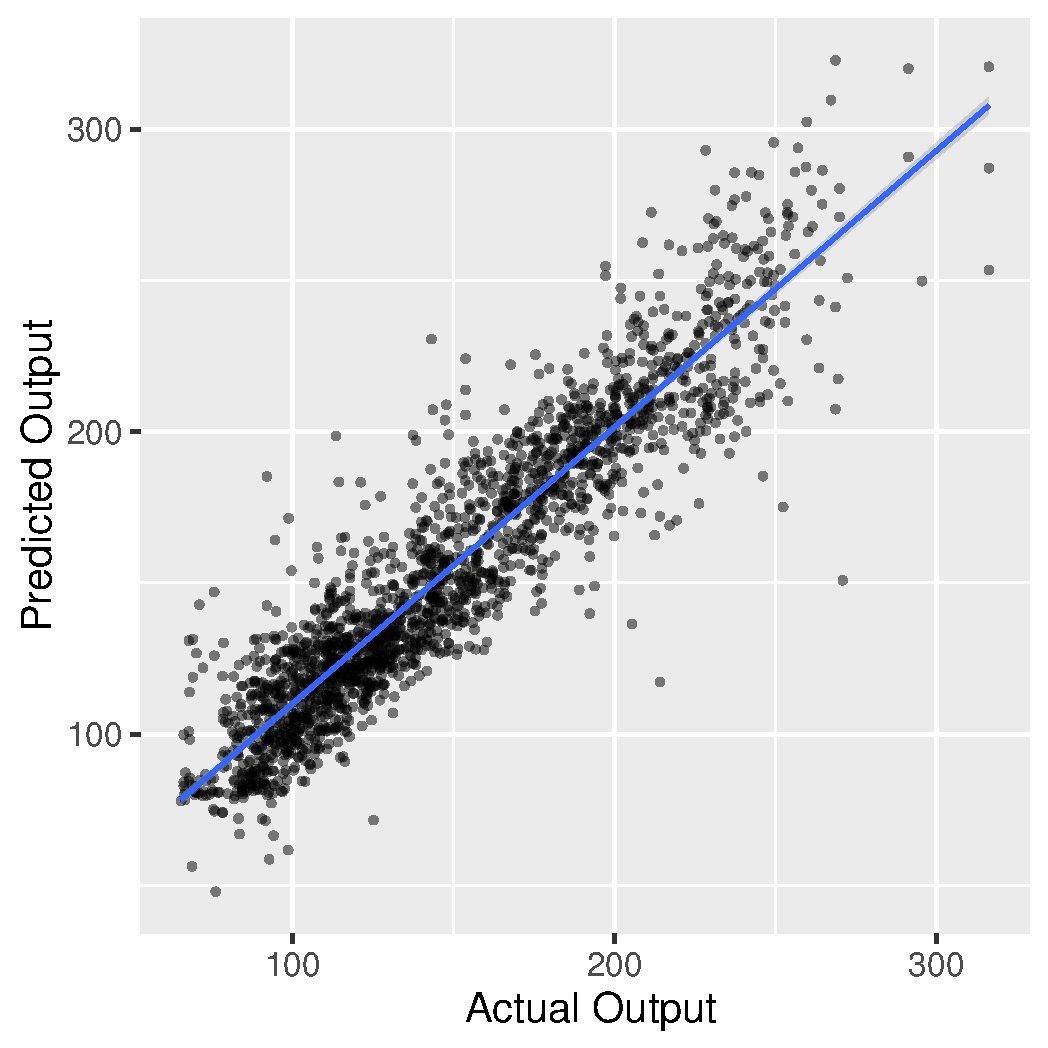
\includegraphics[width=\textwidth]{figures/exp2_scatter_v_test}
    \caption{ \textbf{Problem II}, Goodness of fit, Output $y(x)$}
    \label{fig:problem2_fitv}
  \end{subfigure}
  \hfill
  \begin{subfigure}[b]{0.4\textwidth}
    \centering
    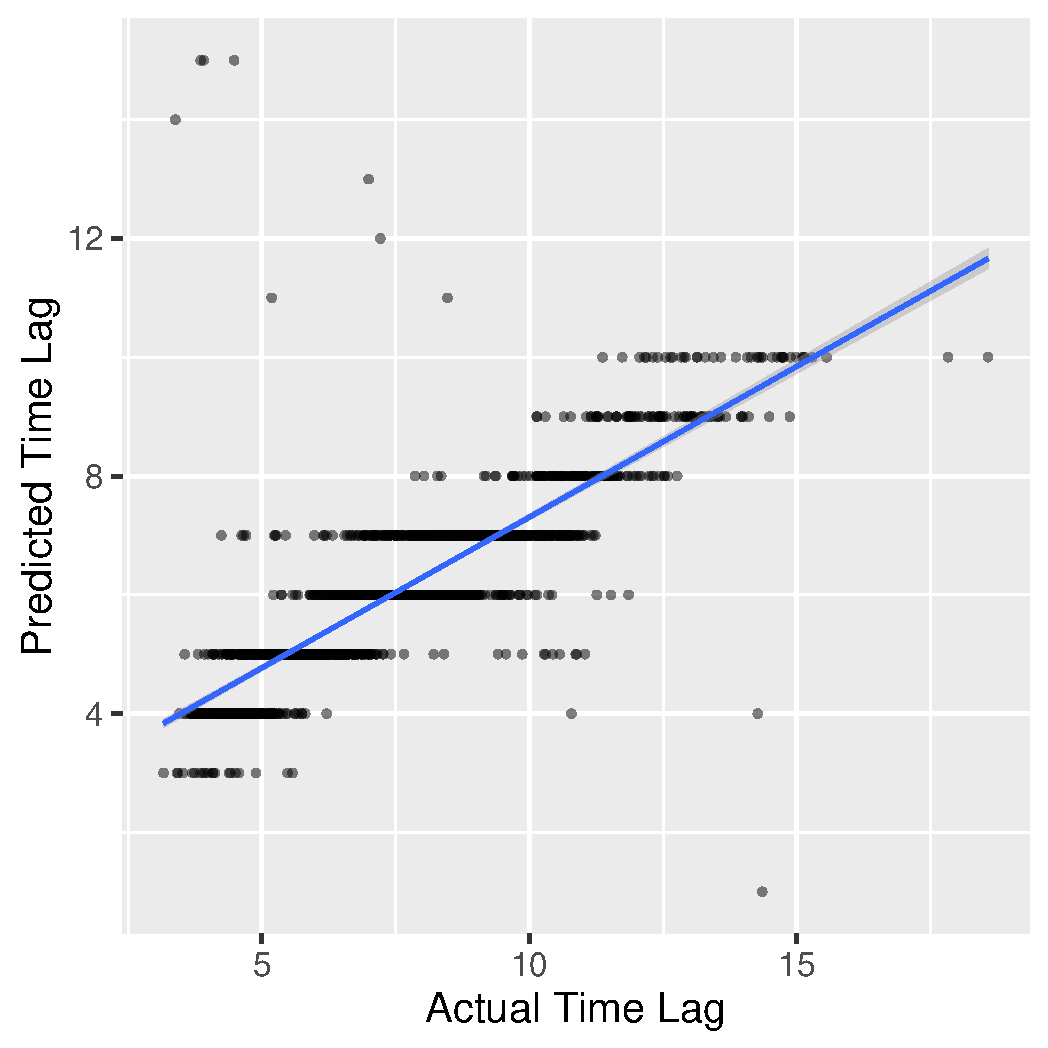
\includegraphics[width=\textwidth]{figures/exp2_scatter_t_test}
    \caption{ \textbf{Problem II}, Goodness of fit, Time lag $\tau(t)$ }
    \label{fig:problem2_fitt}
  \end{subfigure}
  
  \vskip\baselineskip
  
  \begin{subfigure}[b]{0.4\textwidth}
    \centering
    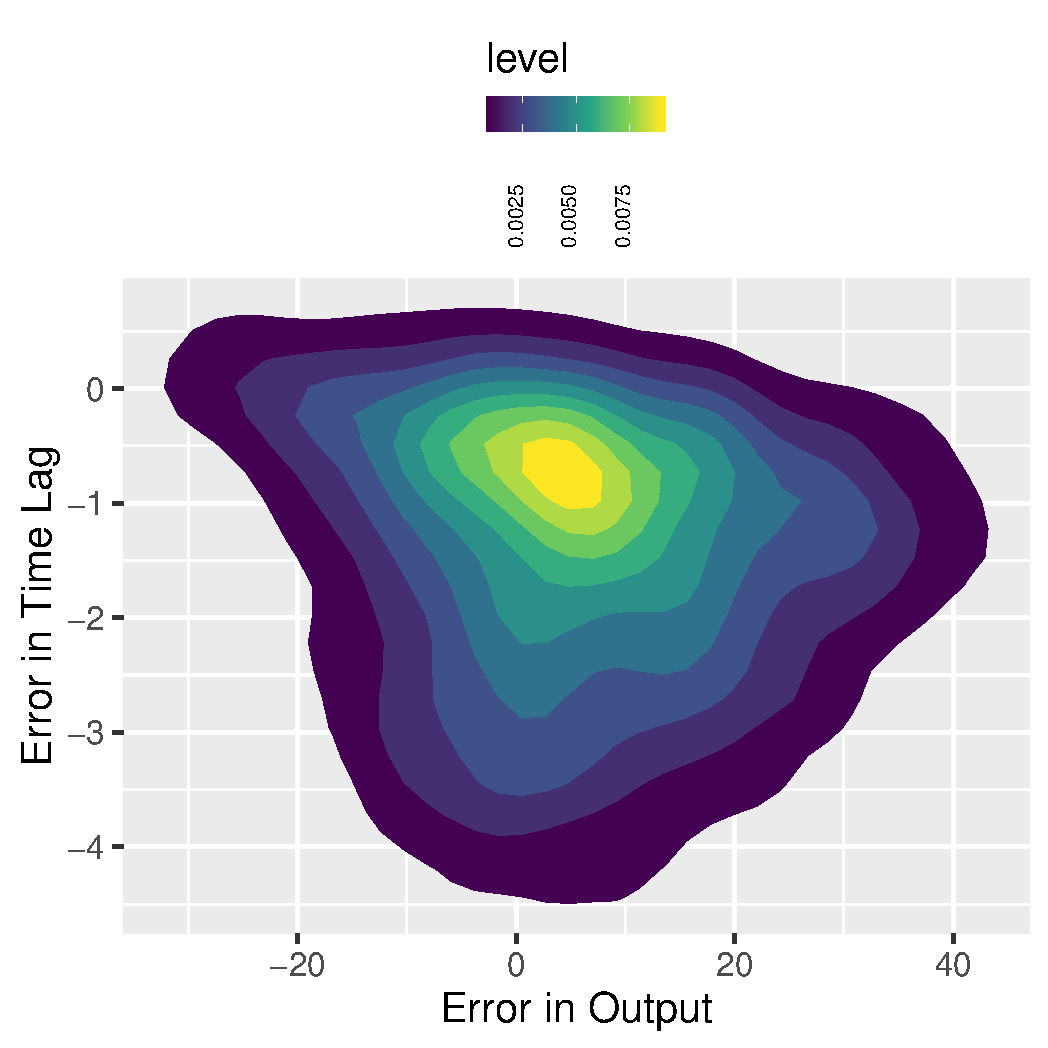
\includegraphics[width=\textwidth]{figures/exp2_errors}
    \caption{ \textbf{Problem II}, Error in prediction of output vs error in time lag prediction} 
    \label{fig:problem2_error}
  \end{subfigure}
  \hfill
  \begin{subfigure}[b]{0.4\textwidth}
    \centering
    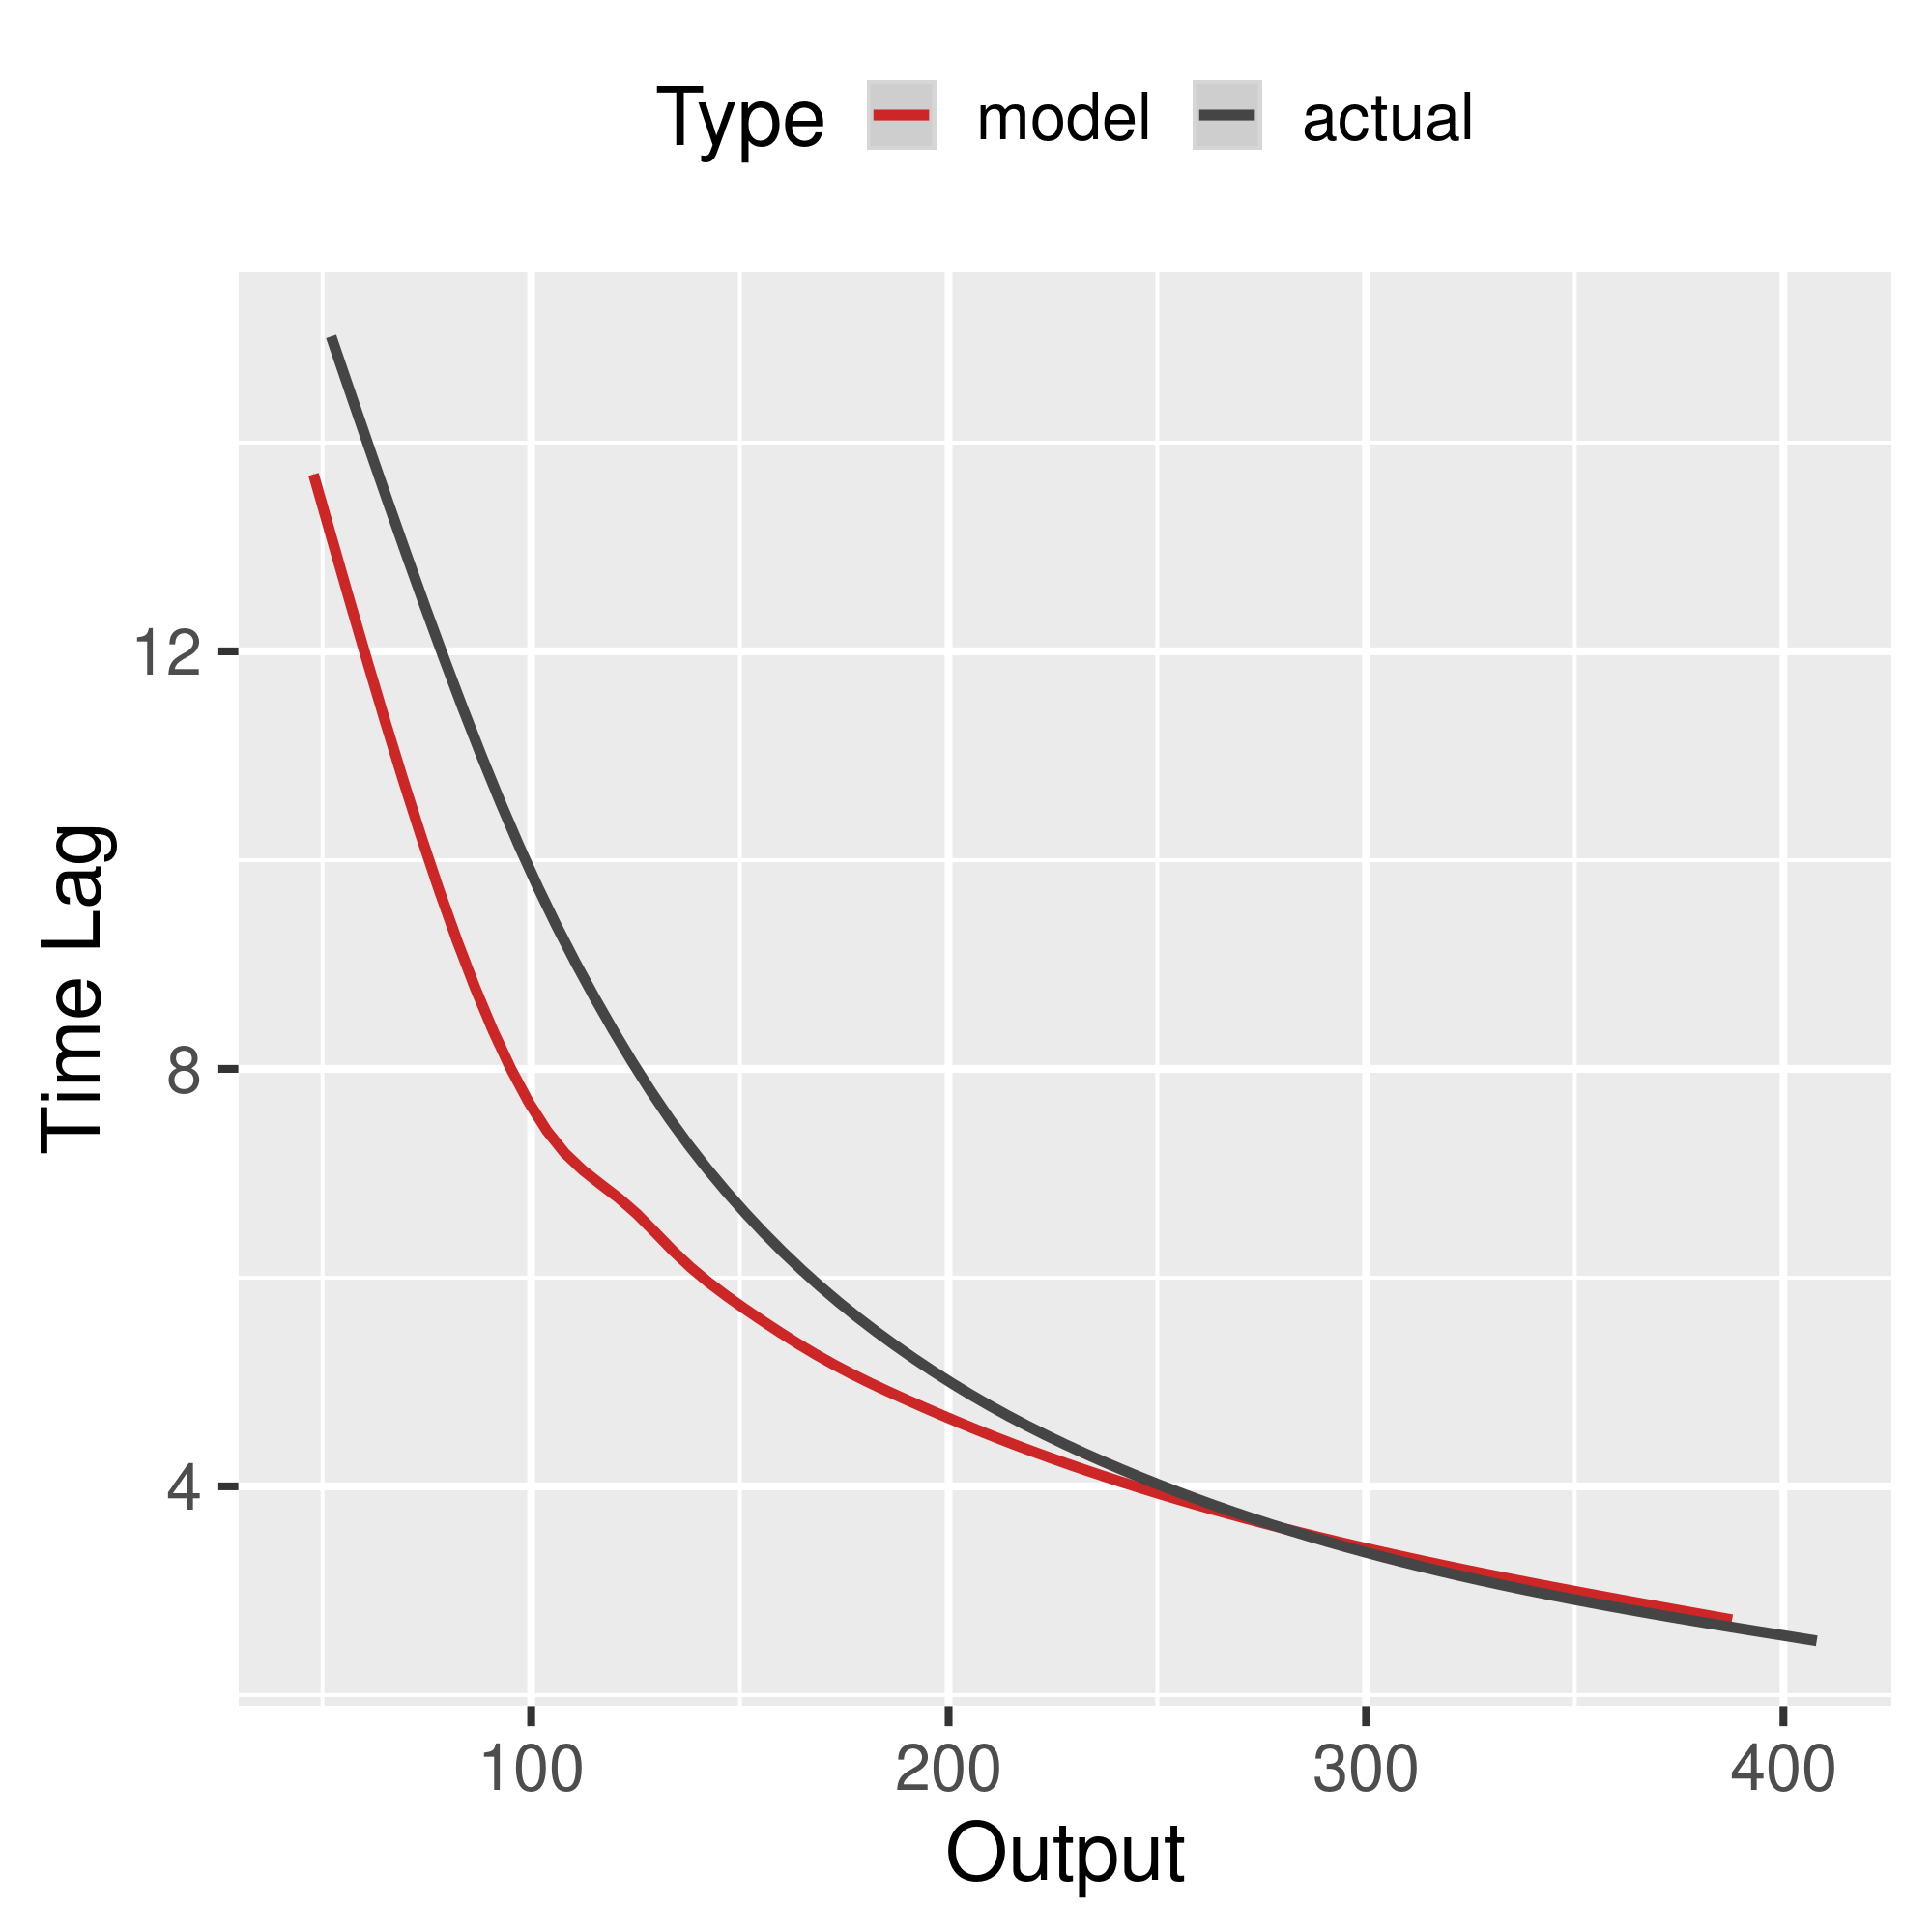
\includegraphics[width=\textwidth]{figures/exp2_predictive_curves}
    \caption{ \textbf{Problem II}, Output vs Time Lag Relationship} 
    \label{fig:problem2_curves}
  \end{subfigure}

  %\vskip\baselineskip
  
  %\begin{subfigure}[b]{0.4\textwidth}
  %  \centering
  %  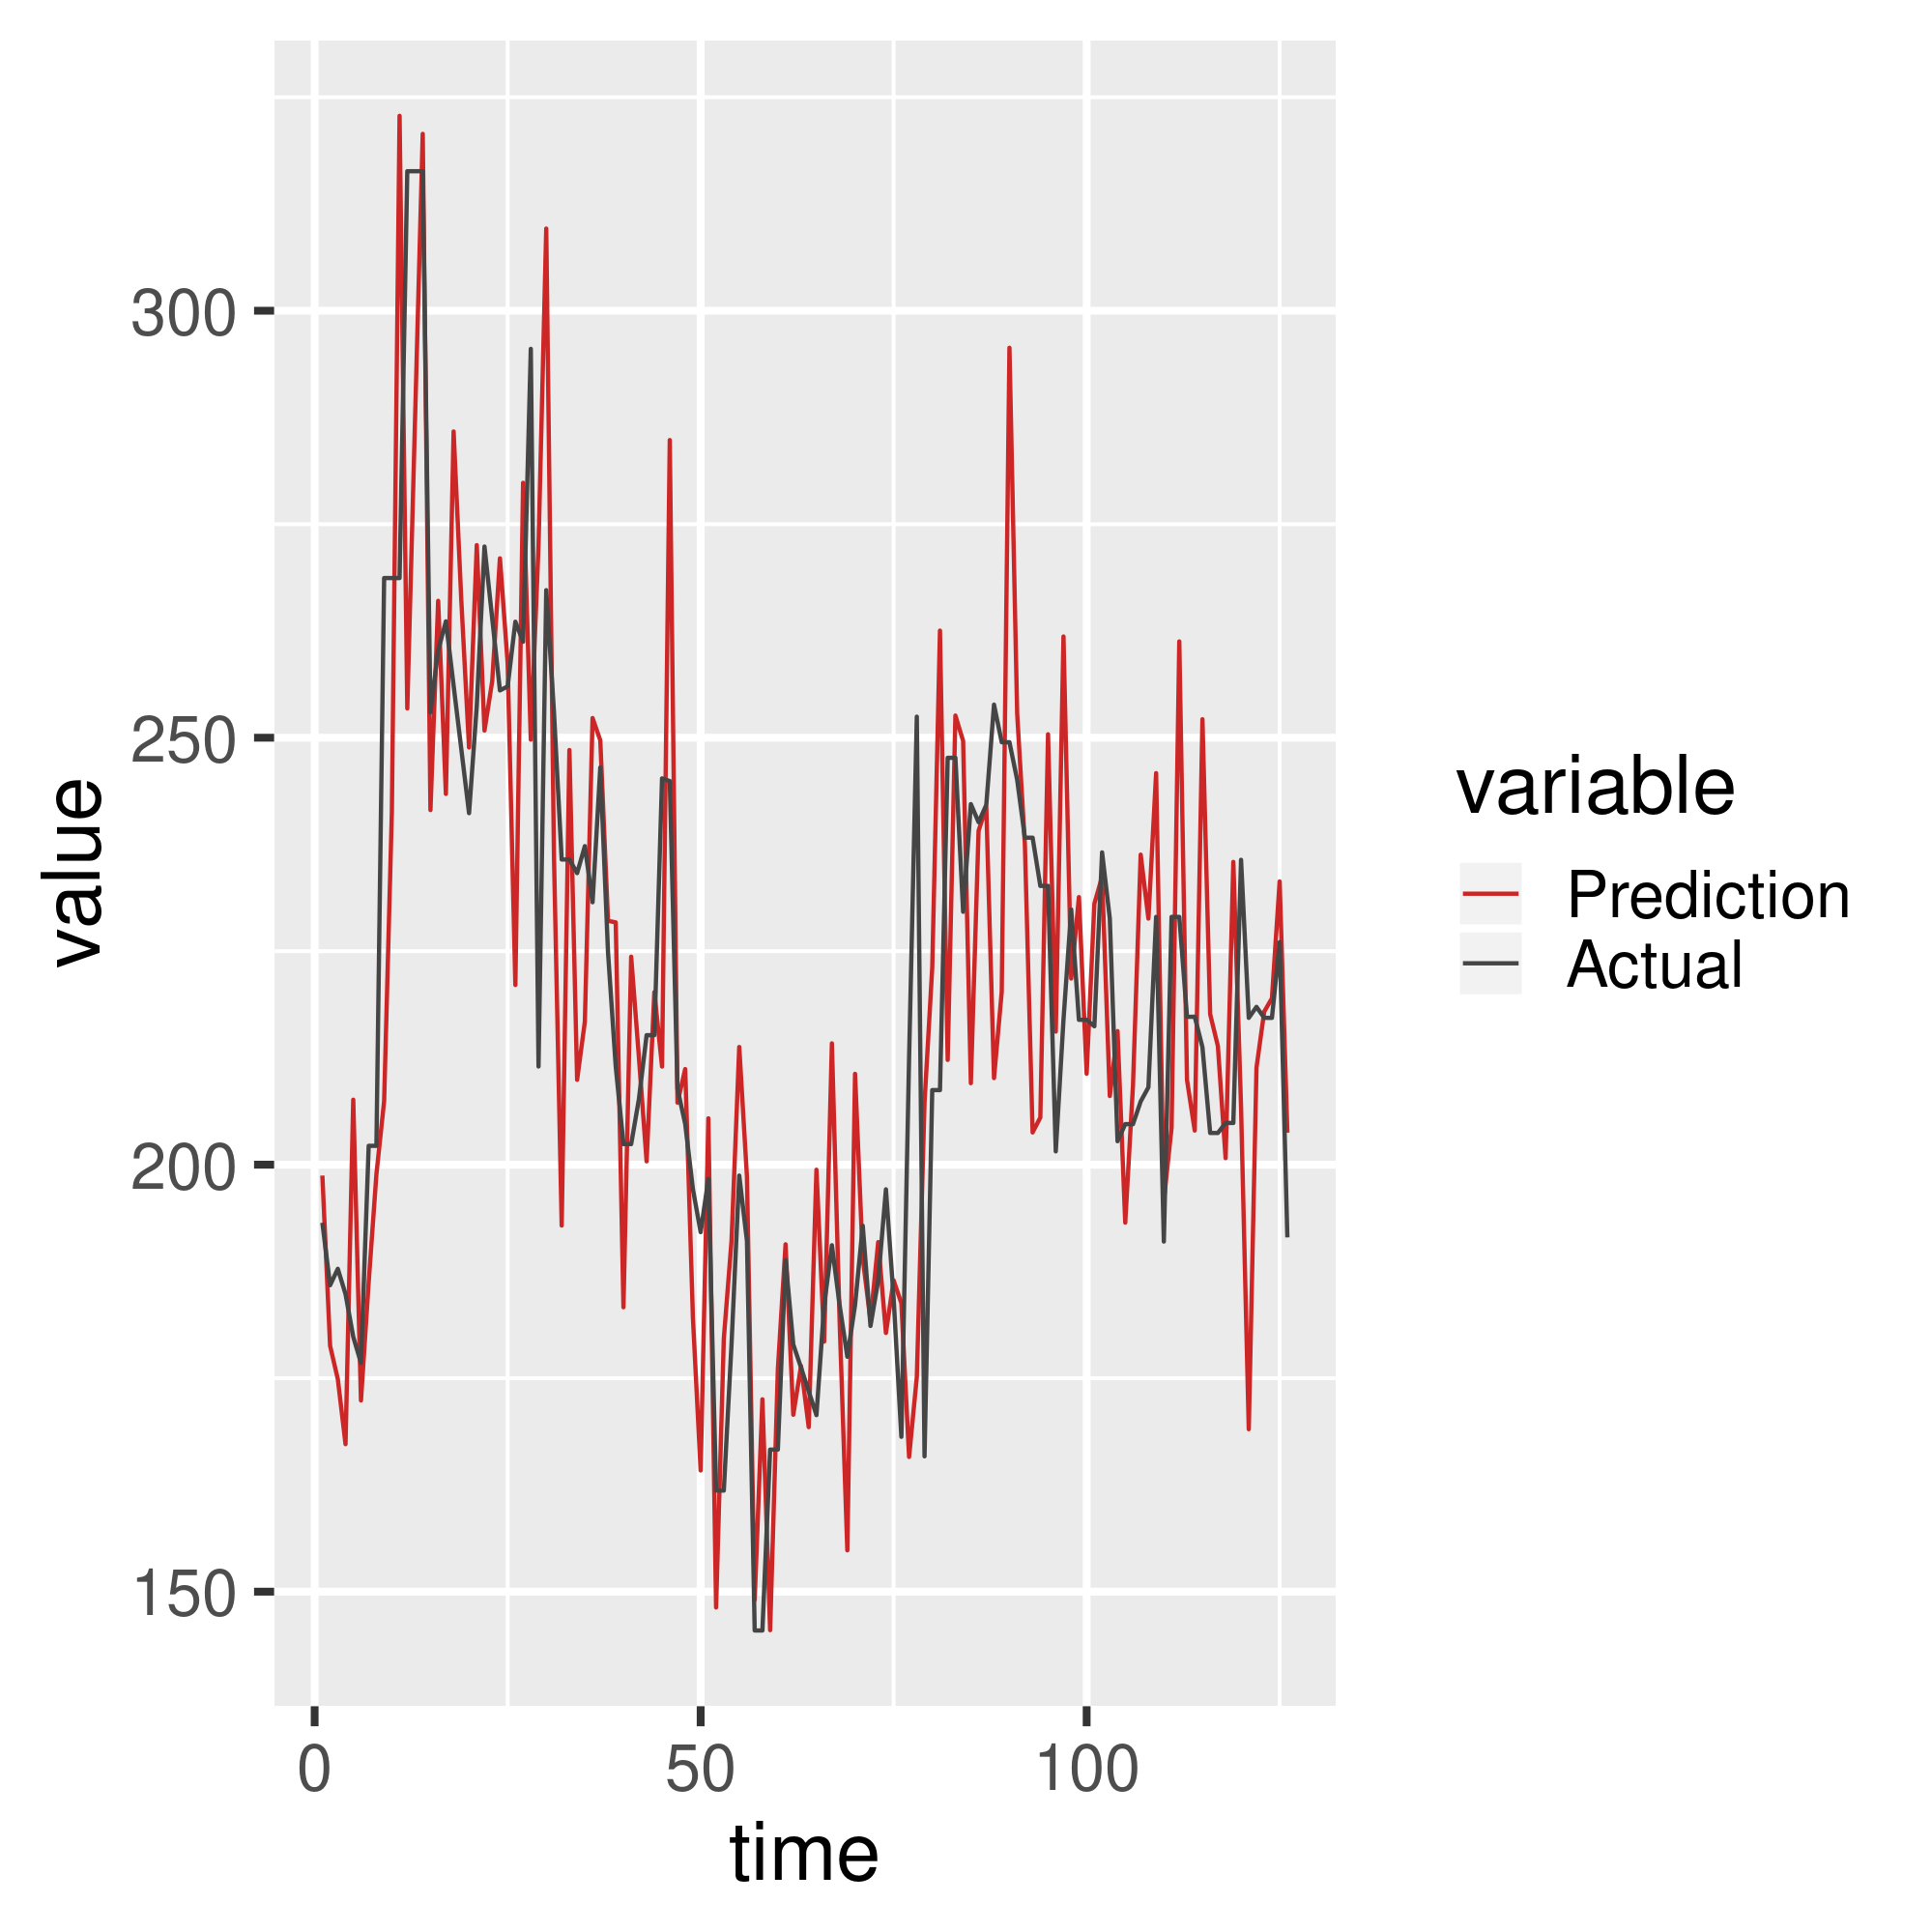
\includegraphics[width=\textwidth]{figures/exp2_timeseries_pred}
  %  \caption{ \textbf{Problem II}, A portion of the test time series reconstructed using the model} 
  %  \label{fig:problem2_timeseries}
  %\end{subfigure}
  %\hfill
  %\begin{subfigure}[b]{0.4\textwidth}
  %  \centering
  %  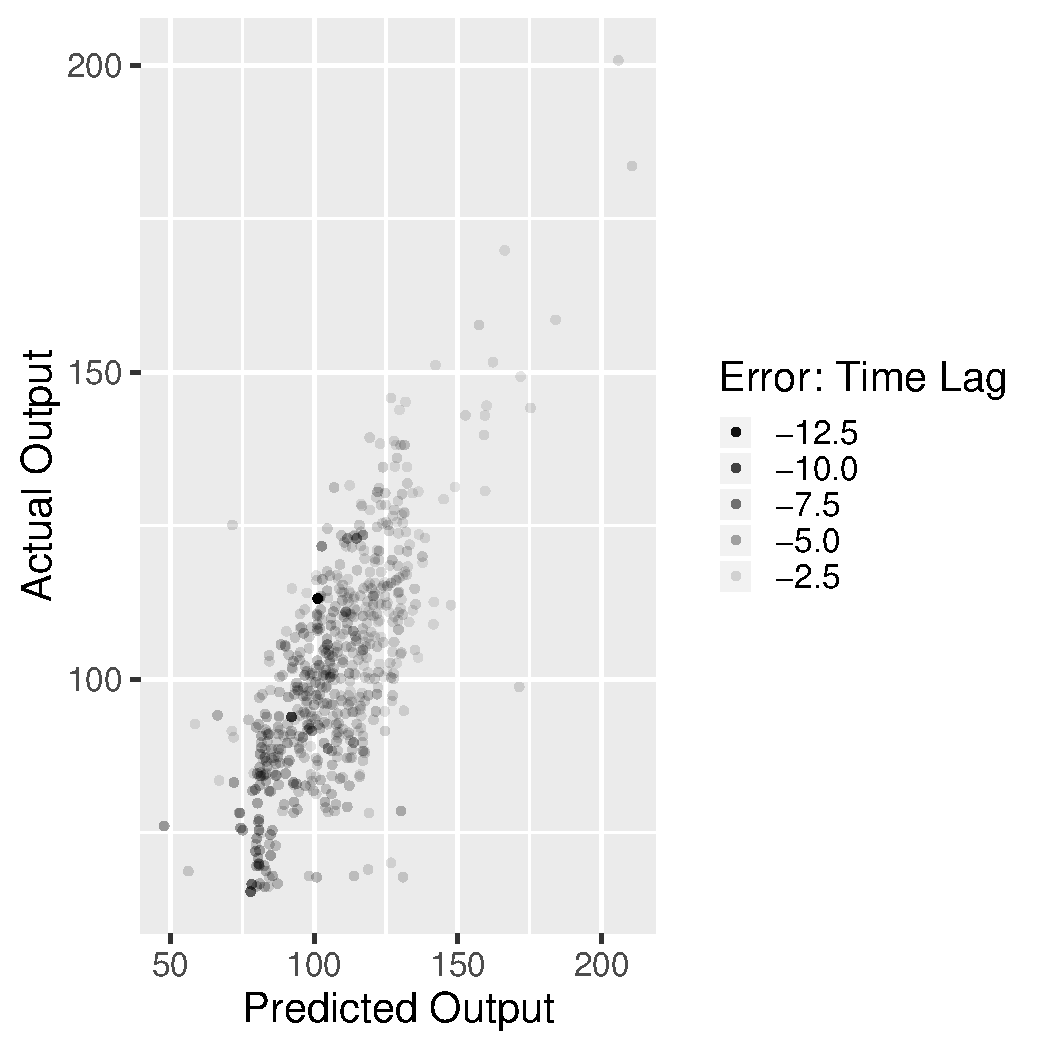
\includegraphics[width=\textwidth]{figures/exp2_lag_error_jus}
  %  \caption{ \textbf{Problem II}, Predicted vs Actual Outputs for the cases with time lag error $\leq -2.5$.} 
  %  \label{fig:problem2_lag_error_jus}
  %\end{subfigure}
  
  \caption{\textbf{Problem II}, Results}
\end{figure*}




\subsubsection{Problem II}

Figures \ref{fig:problem2_fitv} and \ref{fig:problem2_fitt} show that the model is able to 
make accurate predictions for the output as well as time lag.

Figure \ref{fig:problem2_curves} presents smoothed trends extracted from the data presented in 
\ref{fig:problem2_fitv}, the red curve represents the output time lag function learned by the model 
while the black curve is the \emph{ground truth} dependence between the two. The model is able to 
approximate the inverse relationship between the output and time lag from the training data.


\begin{figure*}
  \centering

  \begin{subfigure}[b]{0.4\textwidth}
    \centering
    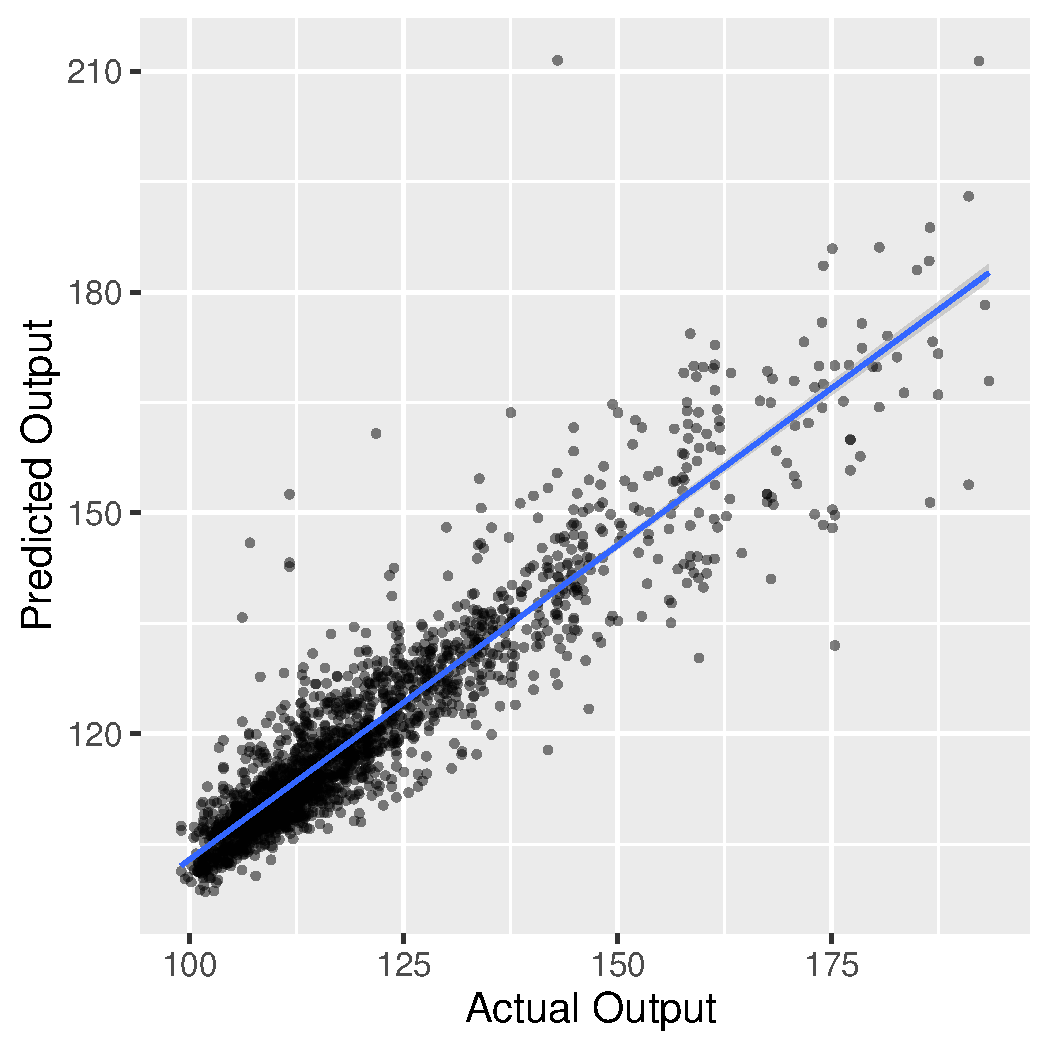
\includegraphics[width=\textwidth]{figures/exp3_scatter_v_test}
    \caption{ \textbf{Problem III}, Goodness of fit, Output $y(x)$}
    \label{fig:problem3_fitv}
  \end{subfigure}
  \hfill
  \begin{subfigure}[b]{0.4\textwidth}
    \centering
    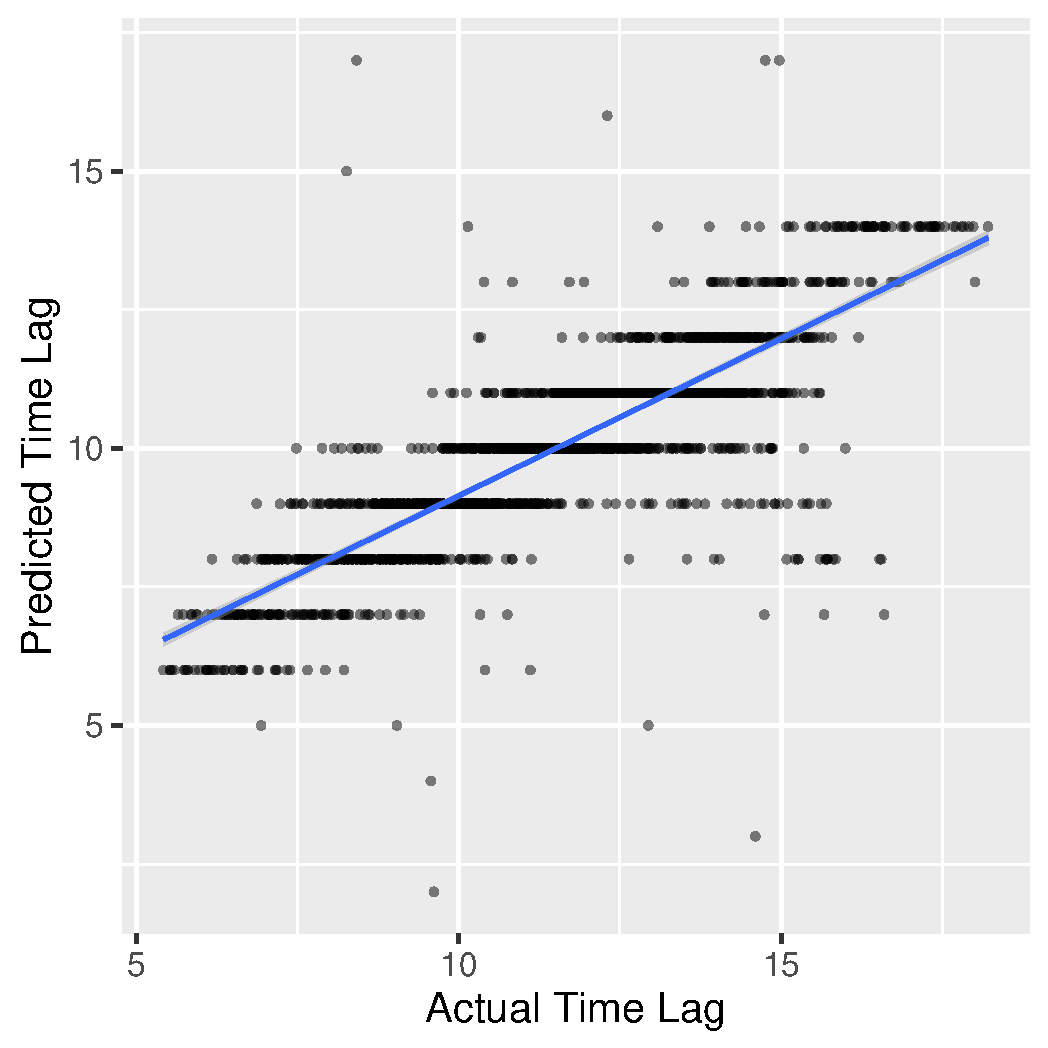
\includegraphics[width=\textwidth]{figures/exp3_scatter_t_test}
    \caption{ \textbf{Problem III}, Goodness of fit, Time lag $\tau(t)$ }
    \label{fig:problem3_fitt}
  \end{subfigure}

  \vskip\baselineskip
  
  \begin{subfigure}[b]{0.4\textwidth}
    \centering
    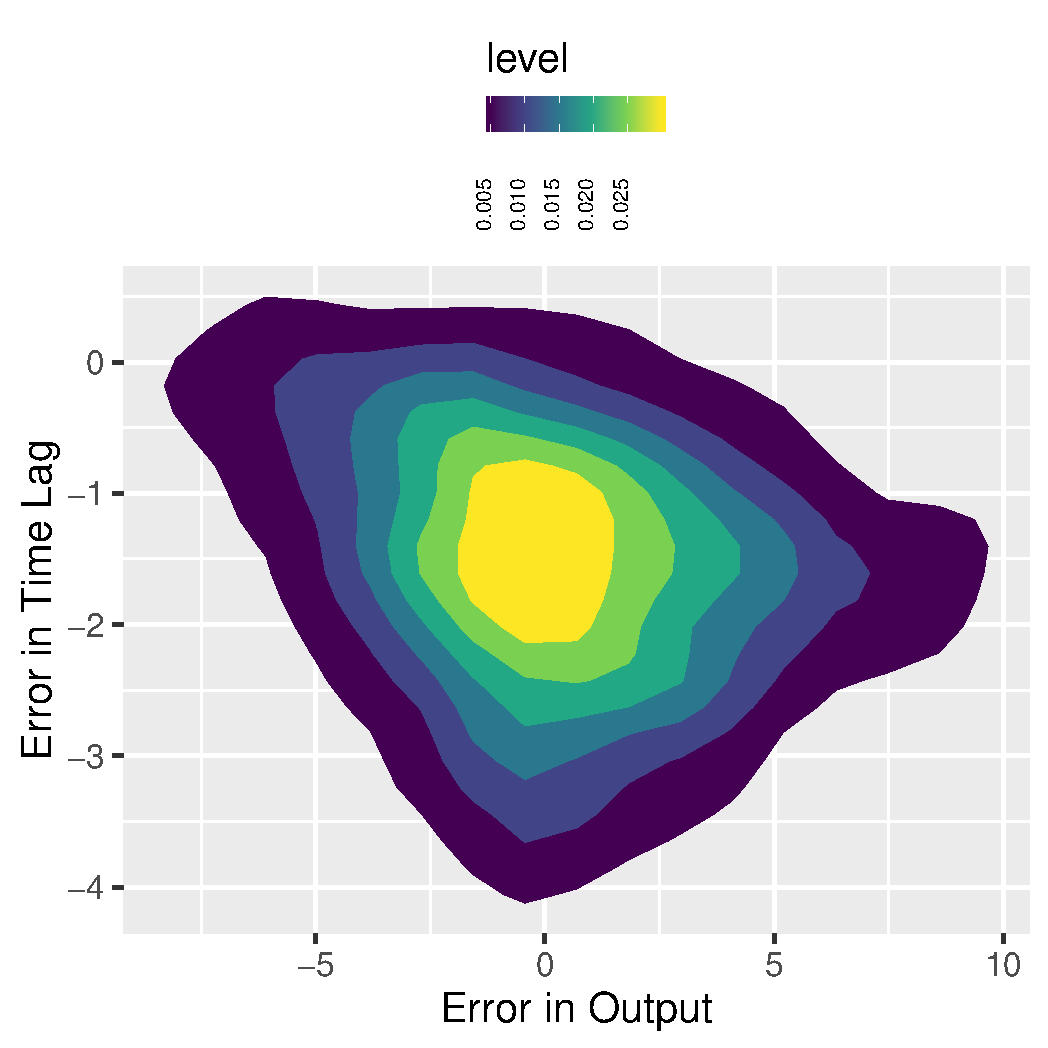
\includegraphics[width=\textwidth]{figures/exp3_errors}
    \caption{ \textbf{Problem III}, Error in prediction of output vs error in time lag prediction} 
    \label{fig:problem3_error}
  \end{subfigure}
  \hfill
  \begin{subfigure}[b]{0.4\textwidth}
    \centering
    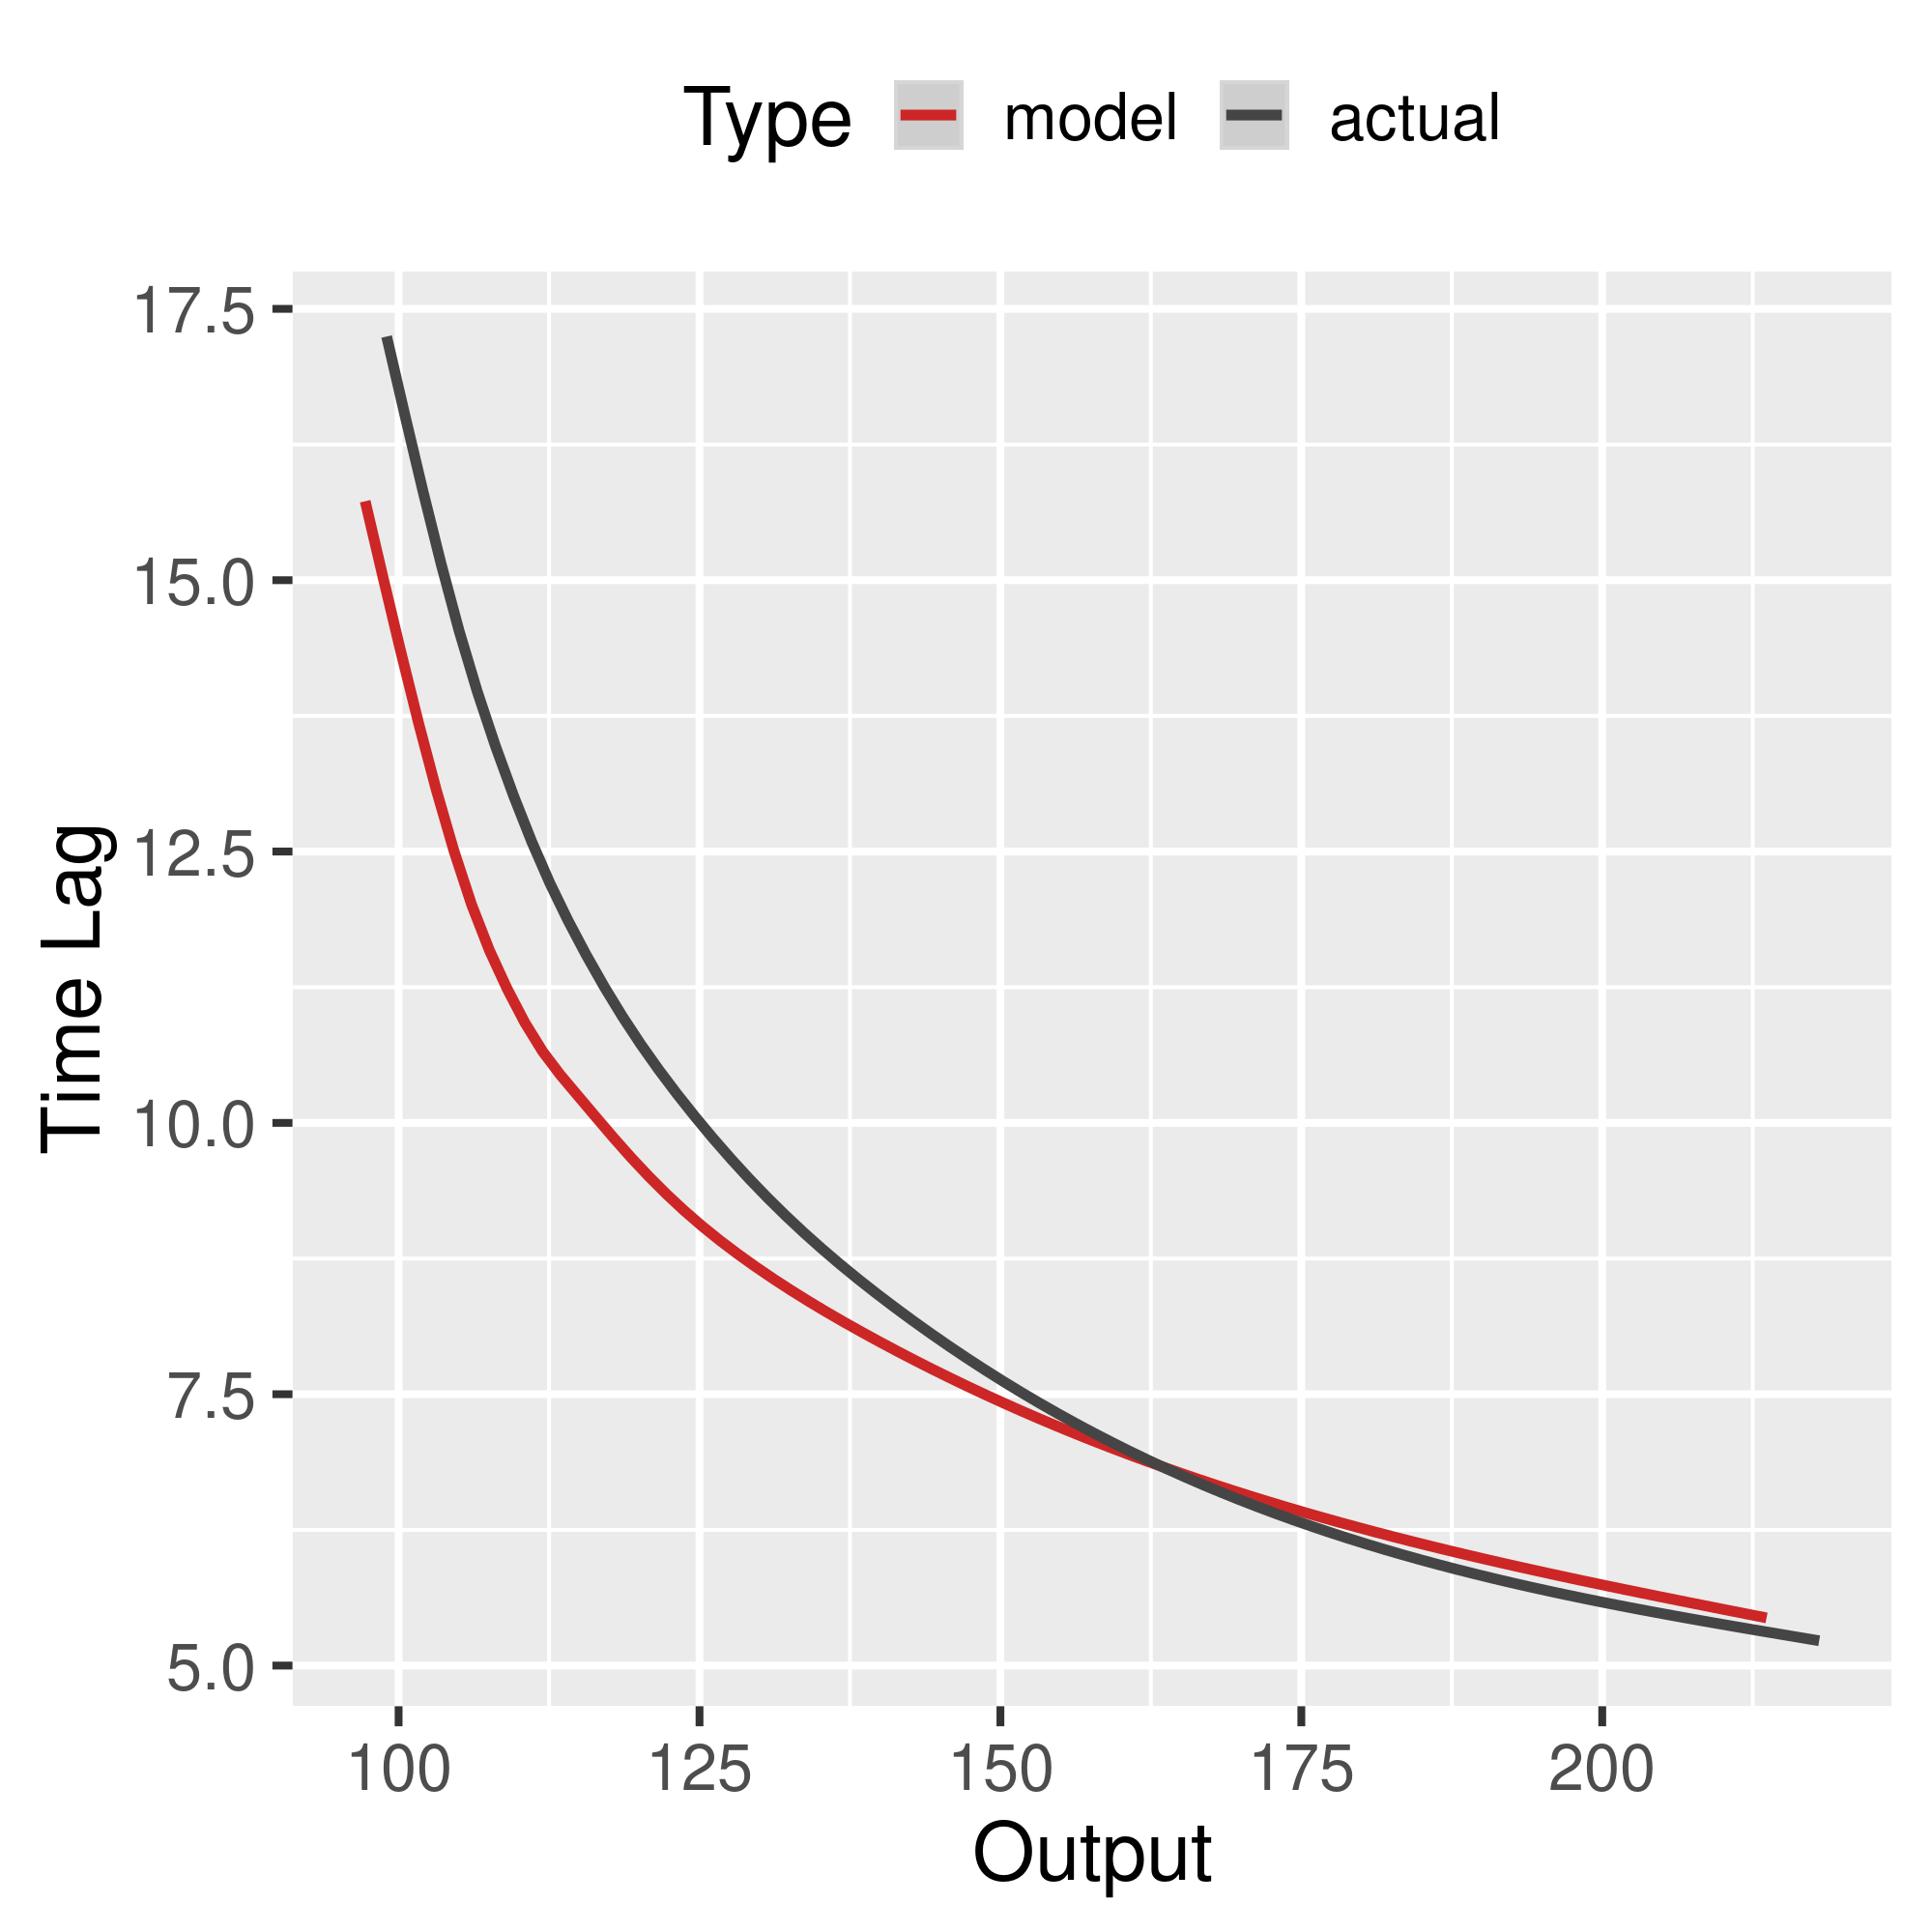
\includegraphics[width=\textwidth]{figures/exp3_predictive_curves}
    \caption{ \textbf{Problem III}, Output vs Time Lag Relationship} 
    \label{fig:problem3_curves}
  \end{subfigure}
  
  %\vskip\baselineskip
  
  %\begin{subfigure}[b]{0.4\textwidth}
  %  \centering
  %  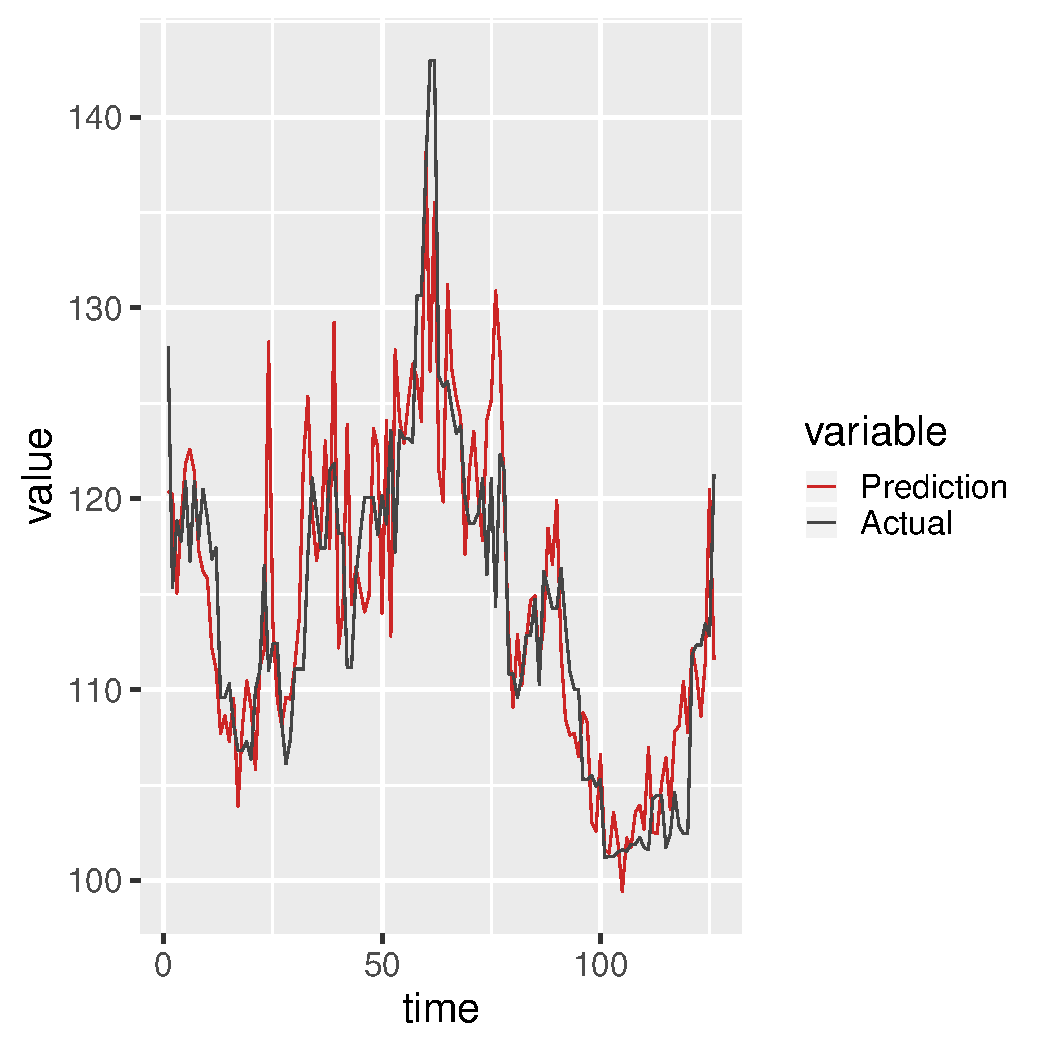
\includegraphics[width=\textwidth]{figures/exp3_timeseries_pred}
  %  \caption{ \textbf{Problem III}, A portion of the test time series reconstructed using the model} 
  %  \label{fig:problem3_timeseries}
  %\end{subfigure}
  %\hfill
  %\begin{subfigure}[b]{0.4\textwidth}
  %  \centering
  %  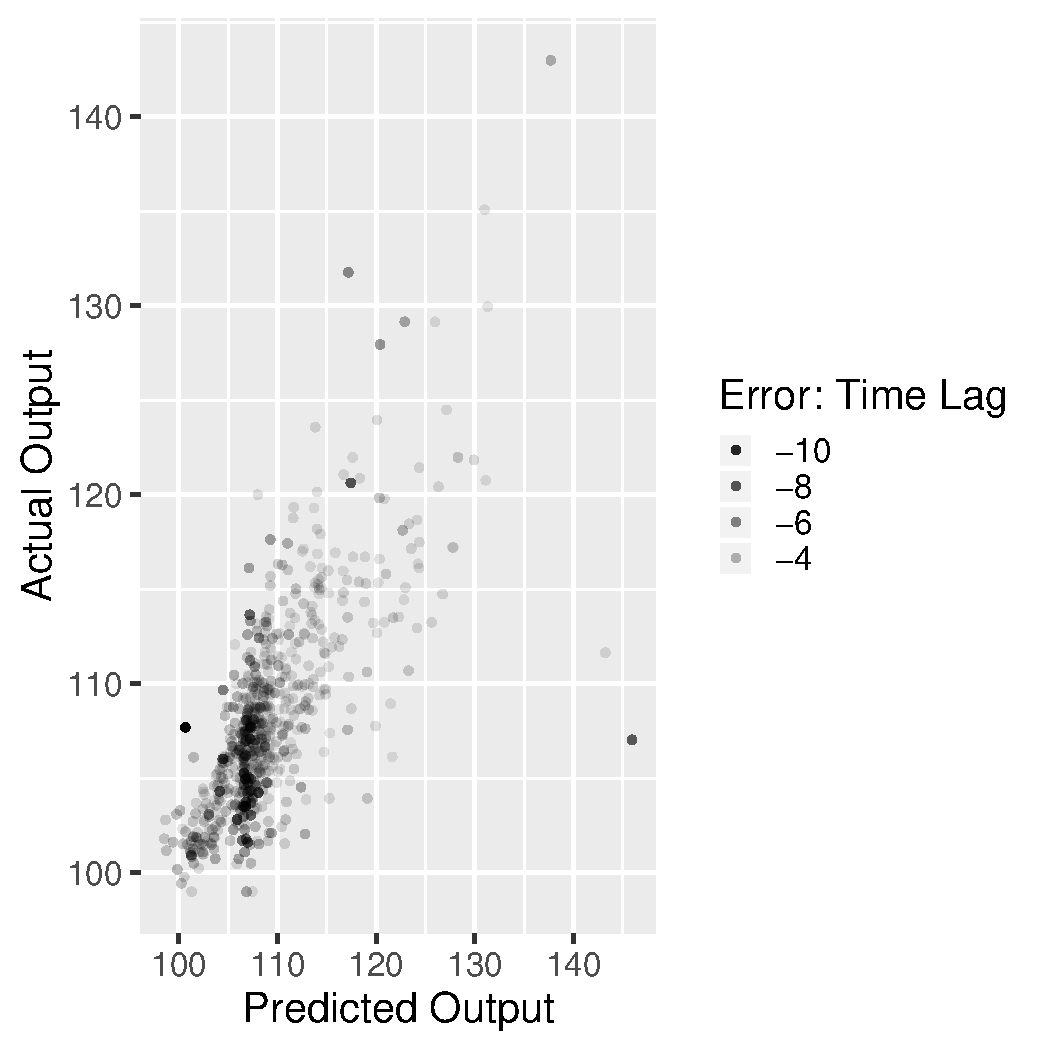
\includegraphics[width=\textwidth]{figures/exp3_lag_error_jus}
  %  \caption{ \textbf{Problem III}, Predicted vs Actual Outputs for the cases with time lag error $\leq -2.5$.} 
  %  \label{fig:problem3_lag_error_jus}
  %\end{subfigure}
  
  \caption{\textbf{Problem III}, Results}
\end{figure*}


\subsubsection{Problem III}

Problem III involves a more complicated output time lag relationship than problem II due to the 
effect of acceleration. From figures \ref{fig:problem3_fitv} and \ref{fig:problem3_fitv}, 
it can be observed that the model can still learn the time lag and output mappings but the 
time lag error distribution (\ref{fig:problem3_error}) has a slightly longer tail as compared to 
figure \ref{fig:problem2_error}.


\subsubsection{Problem IV}

Figures \ref{fig:problem4_fitv}, \ref{fig:problem4_fitt}, \ref{fig:problem4_curves} summarize 
the results of the experiment. This case is different as compared to the previous problems as there 
is now a monotonic relationship between the output and time lag.



\begin{figure*}
  \centering

  \begin{subfigure}[b]{0.4\textwidth}
    \centering
    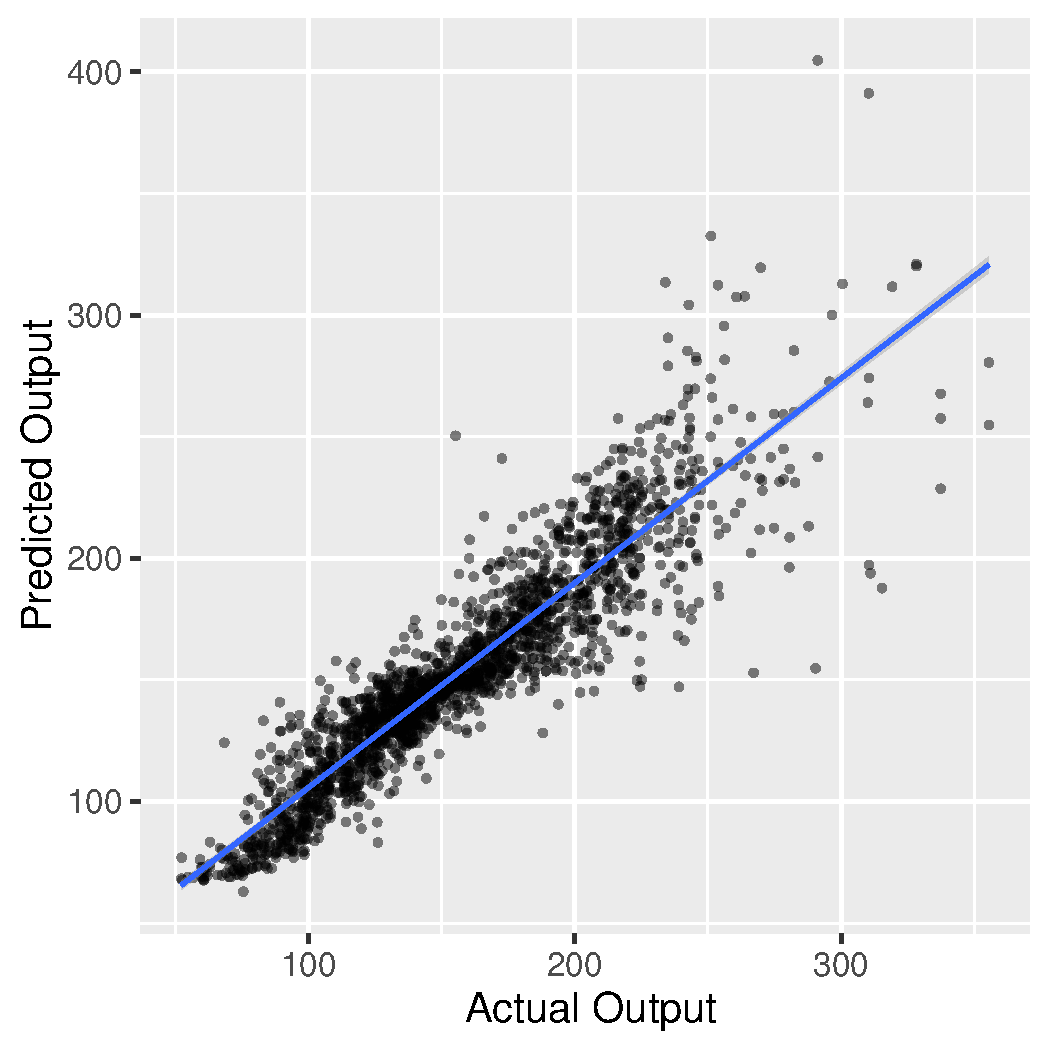
\includegraphics[width=\textwidth]{figures/exp4_scatter_v_test}
    \caption{ \textbf{Problem IV}, Goodness of fit, Output $y(x)$}
    \label{fig:problem4_fitv}
  \end{subfigure}
  \hfill
  \begin{subfigure}[b]{0.4\textwidth}
    \centering
    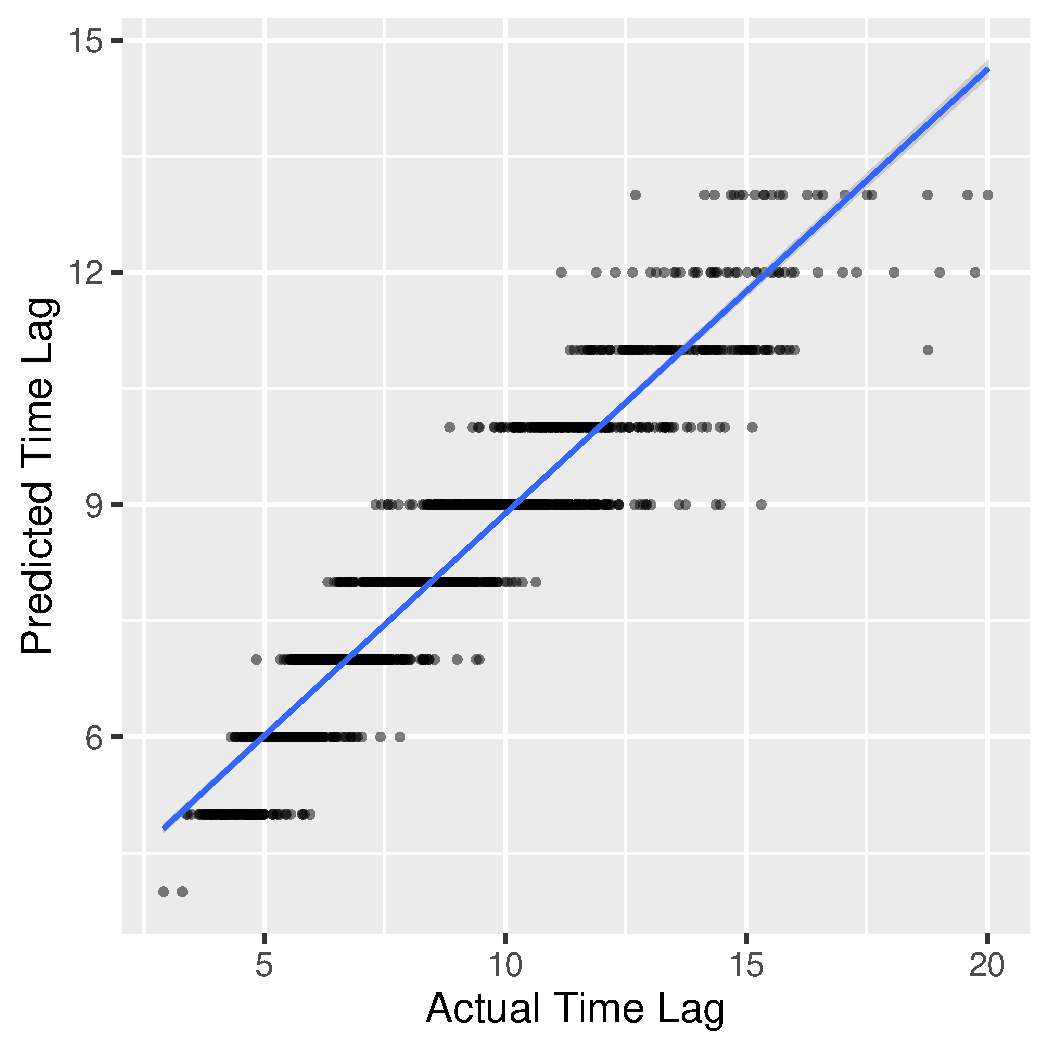
\includegraphics[width=\textwidth]{figures/exp4_scatter_t_test}
    \caption{ \textbf{Problem IV}, Goodness of fit, Time lag $\tau(t)$ }
    \label{fig:problem4_fitt}
  \end{subfigure}
  
  \vskip\baselineskip
  
  \begin{subfigure}[b]{0.4\textwidth}
    \centering
    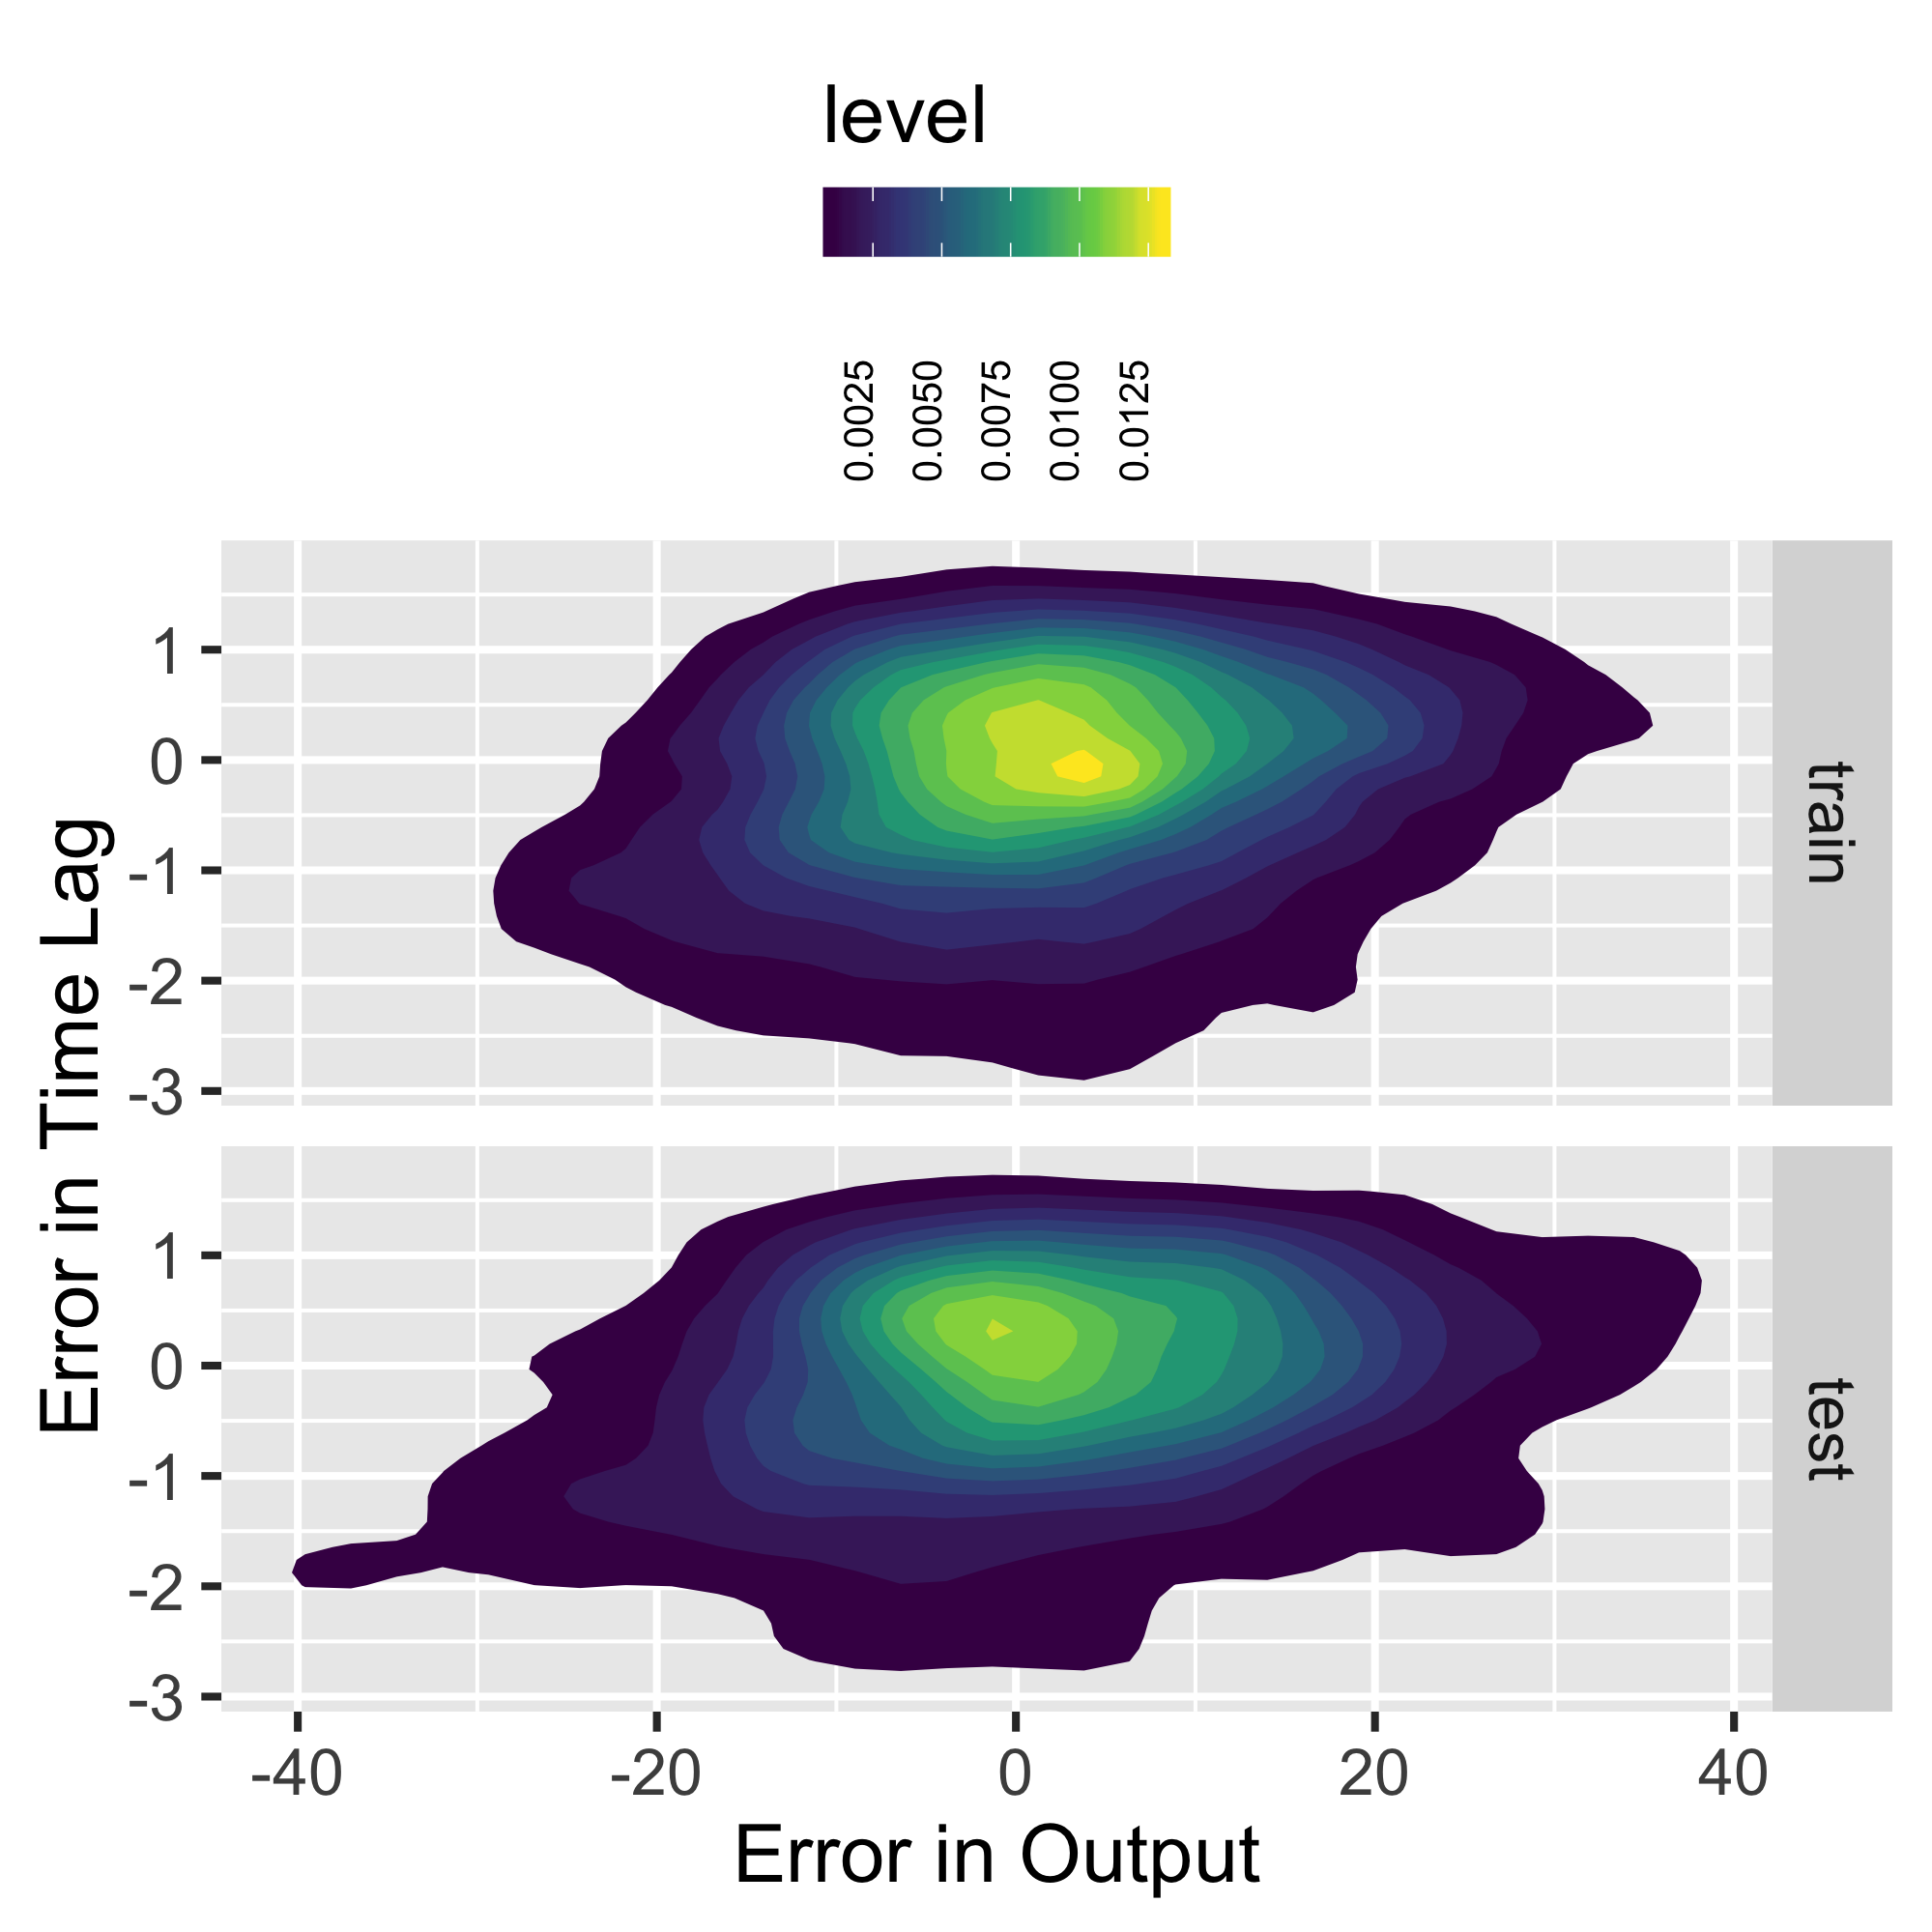
\includegraphics[width=\textwidth]{figures/exp4_errors}
    \caption{ \textbf{Problem IV}, Error in prediction of output vs error in time lag prediction} 
    \label{fig:problem4_error}
  \end{subfigure}
  \hfill
  \begin{subfigure}[b]{0.4\textwidth}
    \centering
    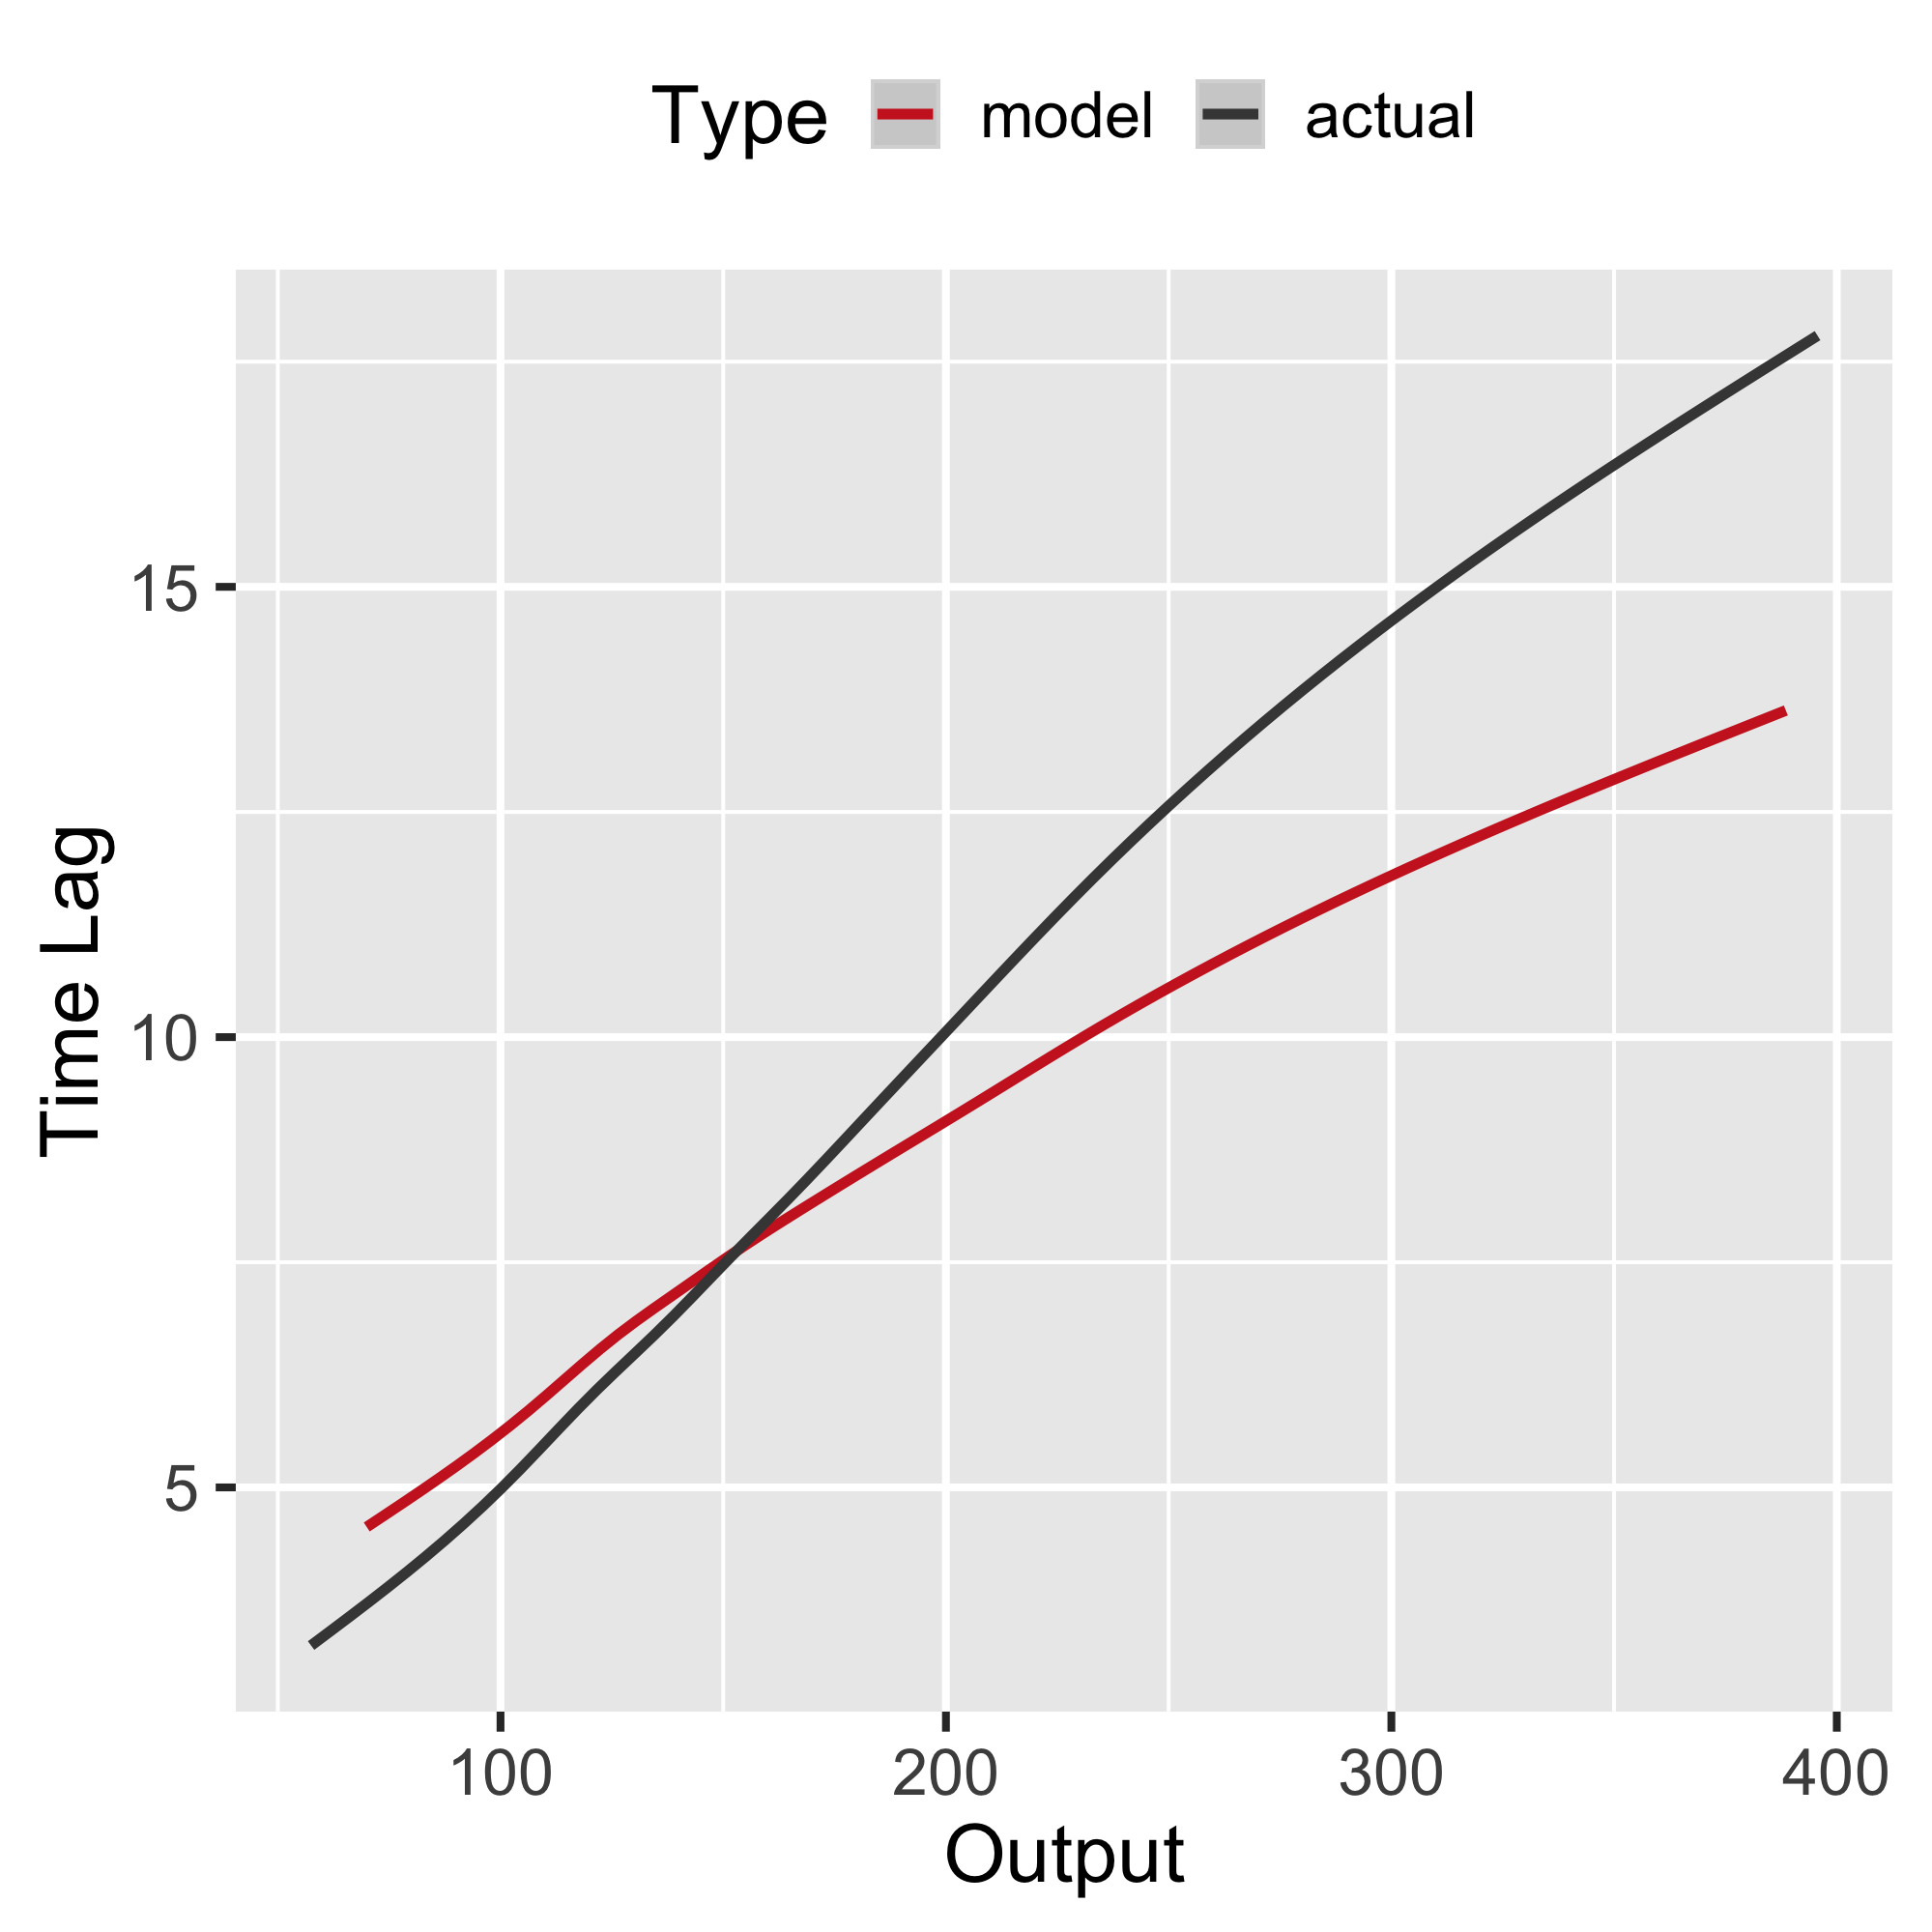
\includegraphics[width=\textwidth]{figures/exp4_predictive_curves}
    \caption{ \textbf{Problem IV}, Output vs Time Lag Relationship} 
    \label{fig:problem4_curves}
  \end{subfigure}
  
  \caption{\textbf{Problem IV}, Results}
\end{figure*}


\subsubsection{Solar Wind Prediction}

Figure \ref{fig:sw_preds} shows observed solar wind speed versus the model's predictions for the test data. 
Although the observed correlation ($0.25$) seems low, this in fact shows a slight improvement above the 
results in \cite{Poduval_2014} where a correlation score of $0.23$ was observed.


\begin{figure}
  \centering
  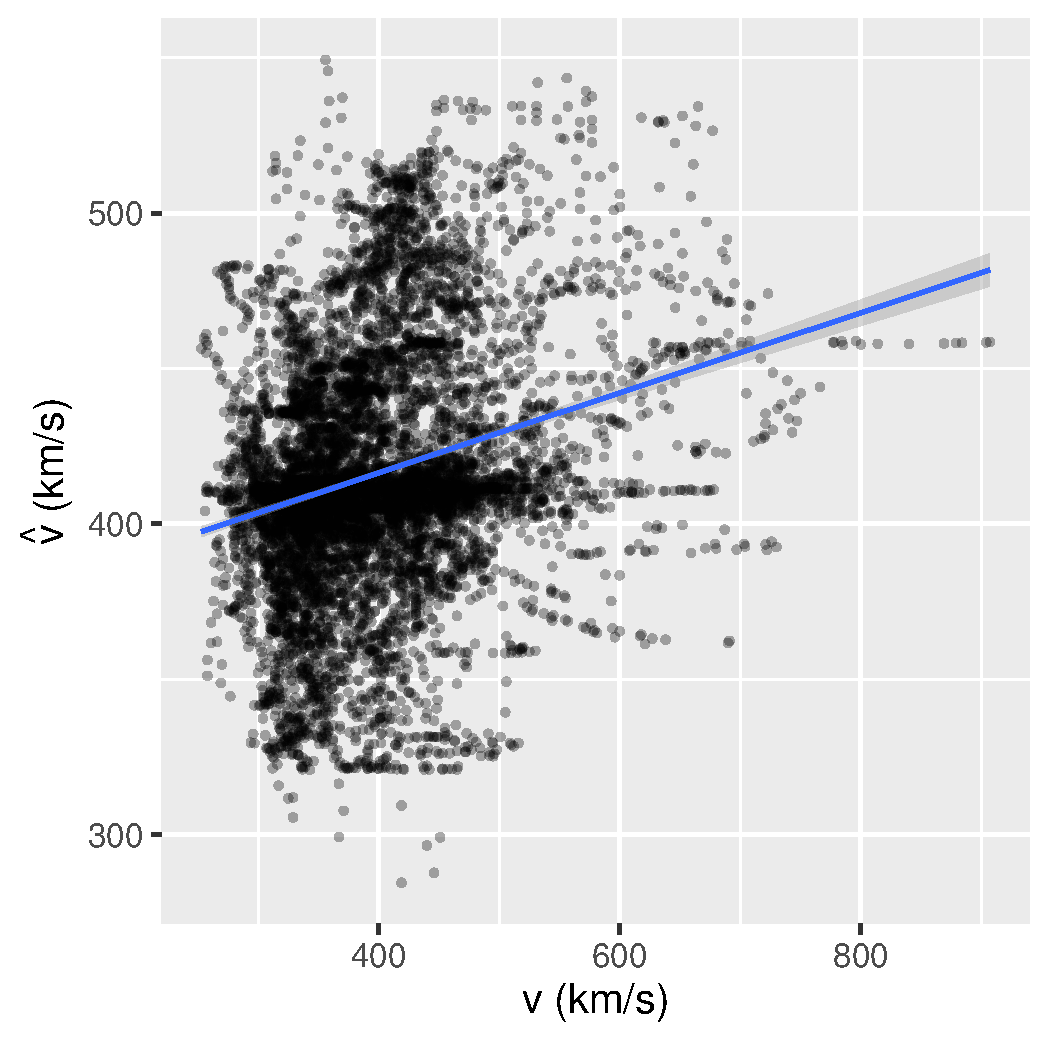
\includegraphics[width=0.5\textwidth]{figures/test_scatter_v}
  \caption{Predicted vs Actual Solar Wind Speed} 
  \label{fig:sw_preds}
\end{figure}


\section{Conclusions}

We present in this work a formulation and a novel solution methodology for the problem of performing 
inference and forecasting in the context of lagged causal relationships between time series. 
We call this problem \emph{Probabilistic Dynamic Time Lag} (PDT) to note the non-stationary nature of the 
causal link between time series $x(t)$ and $y(t)$. 

We outlined a neural network based solution to this problem and benchmark its performance 
on a set of synthetic examples.

Going ahead we plan to augment the FTE data set with other solar data sources to improve
the model's predictive performance on the solar wind forecasting problem.


\subsubsection*{Acknowledgements}

\begin{appendix}
\section{Log likelihood of the latent model~(\ref{eq:py})}\label{app:LL}
Assume that the number of learning samples tends to infinity, and so that in a small volume $dv = dxd{\bf y}$ around a given  joint configuration $(x,{\bf y})$,
the number of data $N_{x,{\bf y}}$ becomes large. Restricting the likelihood to this subset of the data yields the following:
\[
{\cal L}_{x,{\bf y}} = \prod_{m=1}^{N_{x,{\bf y}}} \sum_{\{\tau^{(m)}\}} 
\frac{\hat p(\tau^{(m)}\vert x)}{\prod_{i=1}^n\sqrt{2\pi}\ \sigma_i(\tau^{(m)})}
\exp\Bigl(-\frac{1}{2}\sum_{i=1}^n\frac{\bigl(y_i-\hat y_i(x)\bigr)^2}{\sigma_i(\tau^{(m)})^2}\Bigr).
\]
Upon introducing the relative frequencies:
\[
p_i(x,{\bf y}) = \frac{1}{N_{x,{\bf y}}}\sum_{m=1}^{N_{x,{\bf y}}} \tau_i^{(m)} 
\qquad\text{satisfying}\qquad 
\sum_{i=1}^n p_i(x,{\bf y}) = 1,
\]
the sum over the $\tau_i^{(m)}$ is replaced by a sum over these new variables, with the summand obeying a large deviation principle (see e.g.~\cite{Touchette})
\[
{\cal L}_{x,{\bf y}} \asymp \sum_{{\bf p}} 
\exp\Bigl(-N_{x,{\bf y}} {\cal F}_{x,{\bf y}}\bigl[{\bf p}\bigr]\Bigr)
\]
where the rate function simply reads from Sanov's theorem
\[
{\cal F}_{x,{\bf y}}\bigl[\{p\}\bigr] = n\log(\sigma)+
\sum_{i=1}^n\Bigl[\bigl(y_i-\hat y_i(x)\bigr)^2\frac{1+\sum_j\alpha_{ij}p_j}{2\sigma^2}
-\frac{1}{2}p_i\sum_j\log(1+\alpha_{ji})+p_i\log\frac{p_i}{\hat p_i}\Bigr].
\]
Taking the saddle point for $p_i$ yield as a function of $(x,{\bf y})$ expression~(\ref{eq:hatpi}). Inserting this into ${\cal F}$ and taking
the average over the data set yield the log likelihood~(\ref{eq:LL}) with opposite sign. 
$\hat p$ is also subject of being optimized. We have
\[
\frac{\partial{\cal L}}{\partial \hat p_i(x)} = {\mathbb E}_{data,y}\Bigl[\frac{p_i(x,{\bf y})}{\hat p(x)}-\lambda(x)\Bigr],
\]
with $\lambda(x)$ a Lagrange multiplier to insure that $\sum_i\hat p_i(x)=1$ for any $x$ yielding expression~(\ref{eq:tildep}).


\section{Stability analysis}\label{app:Hessian}
The log likelihood as a function of $r$ and $\alpha$ after inserting the optimal
${\bf p} = {\bf p}(x,{\bf y})$ reads in that case
\[
{\cal L}(r,\alpha) = -\frac{n}{2}\log(r)-\frac{n}{2r}+{\mathbb E}_{data}\Bigl(\log(Z)\Bigr)
\]
with
\[
Z = \sum_i \hat p_i(x)\exp\Bigl(-\frac{\alpha}{2r\sigma_0^2}\Delta y_i^2(x)+\frac{1}{2}\log(1+\alpha)\Bigr).
\]
The gradient reads
\begin{align*}
  \frac{\partial {\cal L}}{\partial r} &= \frac{n}{2r^2}\Bigl(1-r+\frac{\alpha}{n}C_1[{\bf p}]\Bigr),\\[0.2cm]
  \frac{\partial {\cal L}}{\partial \alpha} &= \frac{1}{2(1+\alpha)}-\frac{1}{2r}C_1[{\bf p}],  
\end{align*}
with
\[
C_1[{\bf p}] = \frac{1}{\sigma_0^2}{\mathbb E}_{data}\Bigl(\sum_{i=1}^n p_i(x,{\bf y})\Delta y_i^2(x)\Bigr),
\]
This leads to the following relation at the saddle point:
\begin{align*}
  r &= \frac{n-C_1[{\bf p}]}{n-1}\\[0.2cm]
\alpha &= \frac{n}{n-1}\frac{1-C_1[{\bf p}]}{C_1[{\bf p}]}.
\end{align*}
Let us now compute the Hessian. Denoting
\[
C_2[{\bf p}] = \frac{1}{\sigma_0^4}{\mathbb E}_{data}\Bigl[\sum_{i=1}^n p_i(x,{\bf y})\Bigl(\Delta y_i^2(x)-\sum_{j=1}^np_j(x,{\bf y})\Delta y_j^2(x)\Bigr)^2\Bigr],
\]
we have
\begin{align*}
\frac{\partial^2 {\cal L}}{\partial r^2} &= -\frac{n}{2r^2}\Bigl(1+2\frac{1-r}{r}+\frac{2\alpha}{nr}C_1[{\bf p}]-\frac{\alpha^2}{2nr^2}C_2[{\bf p}]\Bigr)\\[0.2cm]
\frac{\partial^2 {\cal L}}{\partial r\partial \alpha} &=\frac{1}{2r^2}\Bigl(C_1[{\bf p}]-\frac{\alpha}{2r}C_2[{\bf p}]\Bigr)\\[0.2cm]
\frac{\partial^2 {\cal L}}{\partial \alpha^2} &= \frac{1}{4r^2}\Bigl(C_2[{\bf p}]-2C_1^2[{\bf p}]\Bigr). 
\end{align*}
As a result, the Hessian evaluated at the degenerate point $\alpha=0$, $r=1$, $\hat  p_i=1/n$ uniform reads
\[
H =\frac{1}{2}
\left[
  \begin{matrix}
 -n & 1\\[0.4cm] 
 1 & \qquad\DD \frac{C_2}{2}-1
  \end{matrix}
  \right]
\]
where
\[
C_2 = \frac{1}{n\sigma_0^4}{\mathbb E}_{data}\Bigl[\sum_{i=1}^n \Bigl(\Delta y_i^2(x)-\frac{1}{n}\sum_{j=1}^n\Delta y_j^2(x)\Bigr)^2\Bigr].
\]

\section{Proof of Proposition~\ref{prop:opred}}\label{app:opred}
Given $I(x)$ a candidate index function we associate the point-like measure
\[
p_i(x) = \delta_{i,I(x)}.
\]
Written in terms of $p$ the loss function reads
\[
{\cal L}(\hat y,p) = {\mathbb E}_{x,{\bf y}}\Bigl[\sum_{i=1}^n p_i(x)\bigl(y_i-\hat y(x)\bigr)^2\Bigr].
\]
Under~(\ref{eq:py}) (with $\alpha_{ij}=\alpha\delta_{ij}$) the loss is equal to
\[
{\cal L}(\hat y,p) = {\mathbb E}_x\Bigl[\sum_{i=1}^n p_i(x)\Bigl( \bigl(\hat y_i(x)-\hat y(x)\bigr)^2-\hat p_i(x)\frac{\alpha\sigma^2}{1+\alpha}\Bigr)\Bigr]+\sigma^2
\]
The minimization w.r.t. $\hat y$ yields
\begin{equation}\label{eq:hy}
\hat y(x) = \sum_{i=1}^n p_i(x)\hat y_i(x).
\end{equation}
In turn, as a function of $p_i$ the loss being a  convex combination, its minimization yields
\begin{align}
  p_i(x) &= \delta_{i,I(x)},\label{eq:hp}\\[0.2cm]
  I(x) &= \argmin_i\Bigl(\bigl(\hat y_i(x)-\hat y(x)\bigr)^2-\hat p_i(x)\frac{\alpha\sigma^2}{1+\alpha}\Bigr).\label{eq:hI}
\end{align}
Combining these equations~(\ref{eq:hy},\ref{eq:hp},\ref{eq:hI}) we get
\[
I(x) = \argmax_i\bigl(\hat p_i(x)\bigr),
\]
which concludes the proof.  


\end{appendix}


\clearpage
\bibliography{references}

\end{document}
